%!TEX root = ../DSGEnotes.tex
\begin{subappendices}

\section{欧拉公式(复分析)}
\label{sec:euler-complex}

\subsection{欧拉公式和欧拉恒等式}
\label{sec:euler-complex-formula-identityt}

复分析意义上的欧拉公式(Euler formula)\index{Euler formula (complex analysis) \dotfill 欧拉公式}可以表示为
\begin{equation}
  \label{eq:euler-complex-def}
  \exp \left[ i \theta \right] = \cos \theta + i \sin \theta,
\end{equation}
其中$i$是虚数(imaginary number),满足$i = \sqrt{-1}$。欧拉公式的证明,见第\ref{sec:euler-coordinates}节。

欧拉公式的性质,可以从如下引理开始介绍。
\begin{lemma}[$i$的幂是周期方程]
  \label{lemma:i-power-cyclical}
  现在来看$f(x)=i^{x}, \, x=0,1,\ldots$ 的值
  \begin{equation*}
    \begin{pmatrix}
      i^{0}=1, & i^{4}=1, & i^{8}=1, \\
      i^{1}=i, & i^{5}=i, & i^{9}=i, \\
      i^{2}=-1, & i^{6}=-1, & i^{10}=-1, \\
      i^{3}=-i, & i^{7}=-i, & i^{11}=-i, \\
      \vdots & \vdots & \vdots
    \end{pmatrix}
  \end{equation*}
\end{lemma}
不难看出,$i^{x}, \, x=0,1,\ldots$每隔4个数重复一次,因此$f(x)$是一个周期方程。

规律:对于任意整数$x$求$f(x)$,可以将$x$除以$4$,看余数:
\begin{equation*}
  f(x) = i^{n} =
  \begin{cases}
    1 & \text{$\frac{n}{4}$余数是0} \\
    i & \text{$\frac{n}{4}$余数是1} \\
    -1 & \text{$\frac{n}{4}$余数是2} \\
    -i & \text{$\frac{n}{4}$余数是0},
  \end{cases}
\end{equation*}

或者表示为
\begin{equation}
  \label{eq:euler-complex-mod}
  f(x) = i^{x} = i^{x \modd 4}, \, \forall \, x \in \mathcal{Z}.
\end{equation}
其中$\mathcal{Z}_{+}$表示全部正整数集合。$x \modd 4$表示$x$除以4之后的余数。

\begin{lemma}[正弦和余弦的导数]
  \label{lemma:sin-func-derivatives}
现在设$f(x)$是一个正弦函数,满足$f(x)=\sin x$。那么它的$n$次导数,如图\ref{fig:sin-func-derivatives}所示。
\begin{figure}[htbp]
  \caption{正弦函数的导数}
  \centering
  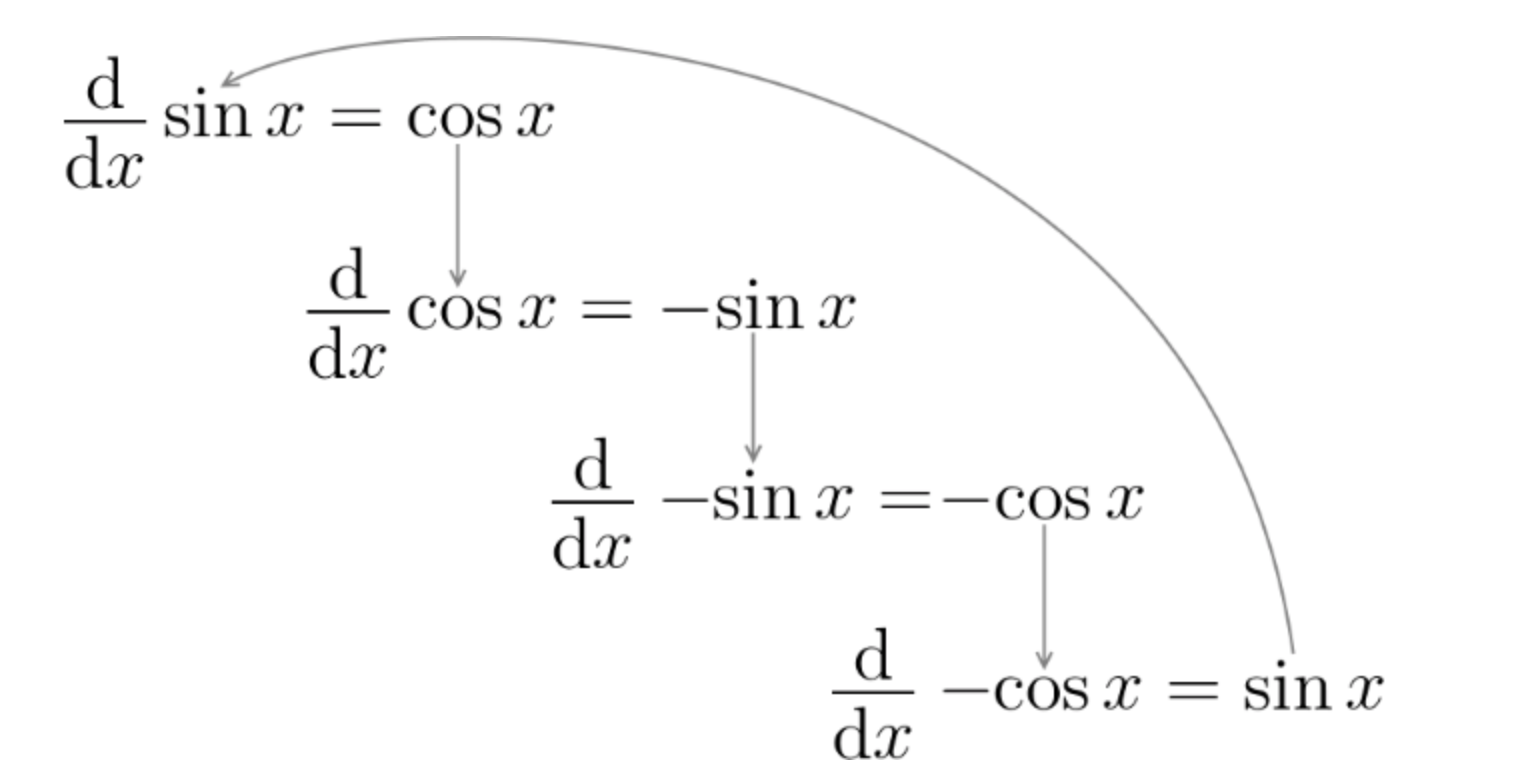
\includegraphics[width=8cm]{./Figures/20180401-sin-cos-derivatives}
  \label{fig:sin-func-derivatives}
%
%  \small{Source: PBOC.}
\end{figure}

\end{lemma}

不难看出,三角函数如正弦的$n$次导数,也是一个以$4$个数为一个周期的周期方程,可以表示为
\begin{equation}
  \label{eq:sin-func-derivatives-mod}
  f^{(n)}(x) = \frac{\mathrm{d}^{n} \sin x}{\mathrm{d} x^{n}}
  = \frac{\mathrm{d}^{n \, \modd \, 4} \sin x}{\mathrm{d} x}
  = \begin{cases}
  \sin x & n \, \modd \, 4 = 0, \\
  \cos x & n \, \modd \, 4 = 1, \\
  - \sin x & n \, \modd \, 4 = 2, \\
  - \cos x & n \,\modd \,4 = 3, \quad \forall \, n \in \mathcal{Z}_{+}.
  \end{cases}
\end{equation}

余弦函数具有类似的性质。此外,对于任意$n \in Z_{+}$,正弦或者余弦函数的$n$阶导数都存在,我们称这种方程为无限可导方程(indefinitely differentiable function)\index{indefinitely differentiable function \dotfill 无限可导方程}。

\begin{lemma}[指数方程的导数]
  \label{lemma:exponential-derivative}
  指数方程的导数是指数方程本身,
  \begin{equation*}
    \frac{\mathrm{d}^{n}}{\mathrm{d} x^{n}} \exp \left[ x \right] = \exp \left[ x \right], \forall \, x, n.
  \end{equation*}
\end{lemma}

\begin{lemma}[泰勒——麦克劳林级数]
  \label{lemma:taylor-maclaurin-series}
  设$f(x)$是一个连续可导方程。对$f(x)$沿着$x=a$做$n$阶的泰勒级数展开,可以得到一个多项式相加的形式,我们称之为泰勒级数(Taylor series)\index{Taylor series \dotfill 泰勒级数}:
  \begin{equation}
    \label{eq:taylor-series-def}
    f \left( x \right) = \frac{f(a)}{0!}
    + \frac{f^{'}(a)}{1!} \left( x - a \right)
    + \frac{f^{''}(a)}{2!} \left( x - a \right)^{2}
    + \ldots
    + \frac{f^{(n)}(a)}{n!} \left( x - a \right)^{n}.
  \end{equation}



%!TEX root = ../DSGEnotes.tex
\begin{figure}[htbp]
  \centering  %居中
  \subfigure[$n=1$]{  %第一张子图
  \begin{minipage}{7cm}
    \centering  %子图居中
    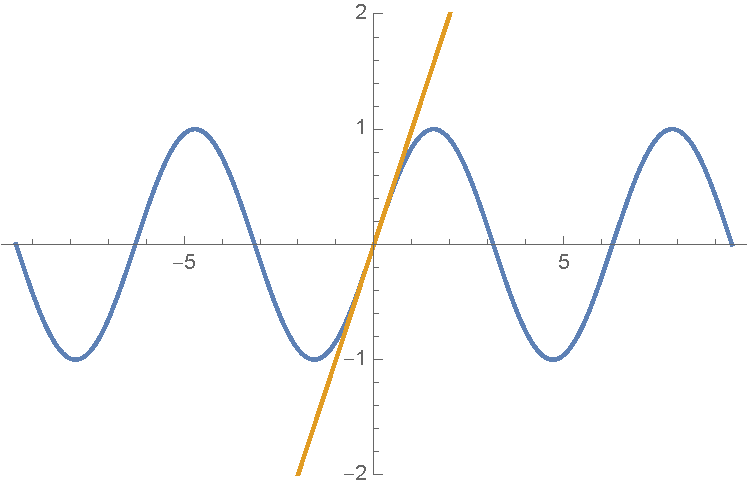
\includegraphics[scale=0.5]{./Figures/20180315-taylor-n1} %以pic.jpg的0.5倍大小输出
  \end{minipage}}
  \subfigure[$n=3$]{  %第二张子图
  \begin{minipage}{7cm}
    \centering  %子图居中
    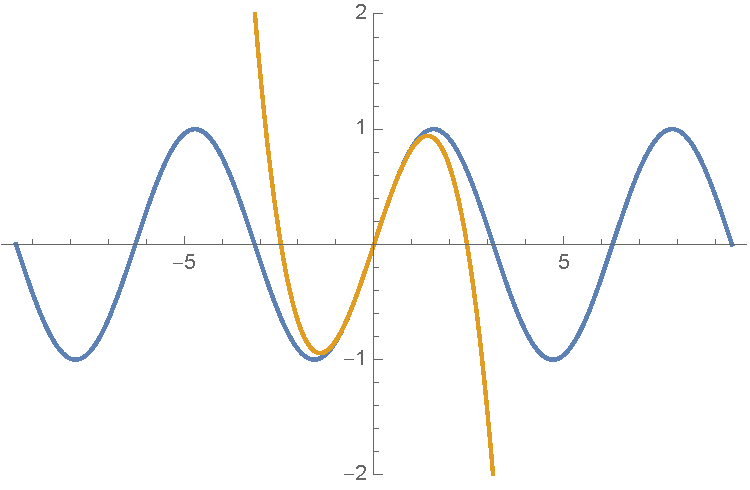
\includegraphics[scale=0.5]{./Figures/20180315-taylor-n3} %以pic.jpg的0.5倍大小输出
  \end{minipage}}
  \subfigure[$n=5$]{  %第二张子图
  \begin{minipage}{7cm}
    \centering  %子图居中
    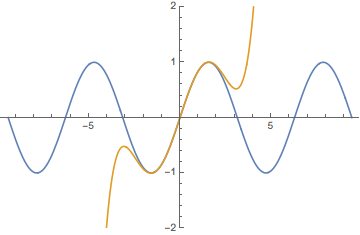
\includegraphics[scale=0.5]{./Figures/20180315-taylor-n5} %以pic.jpg的0.5倍大小输出
  \end{minipage}}
  \subfigure[$n=7$]{  %第二张子图
  \begin{minipage}{7cm}
    \centering  %子图居中
    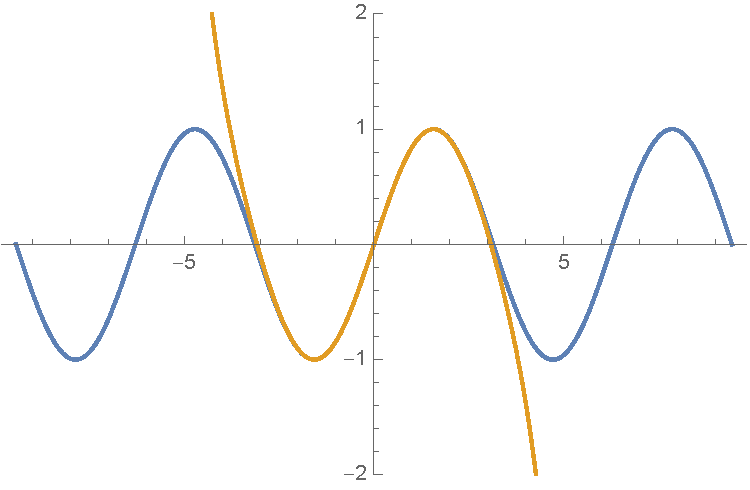
\includegraphics[scale=0.5]{./Figures/20180315-taylor-n7} %以pic.jpg的0.5倍大小输出
  \end{minipage}}
  \subfigure[$n=9$]{  %第二张子图
  \begin{minipage}{7cm}
    \centering  %子图居中
    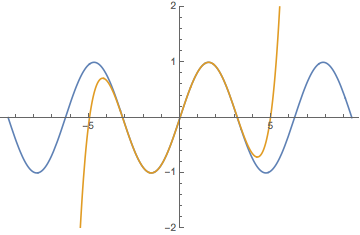
\includegraphics[scale=0.5]{./Figures/20180315-taylor-n9} %以pic.jpg的0.5倍大小输出
  \end{minipage}}
  \subfigure[$n=11$]{  %第二张子图
  \begin{minipage}{7cm}
    \centering  %子图居中
    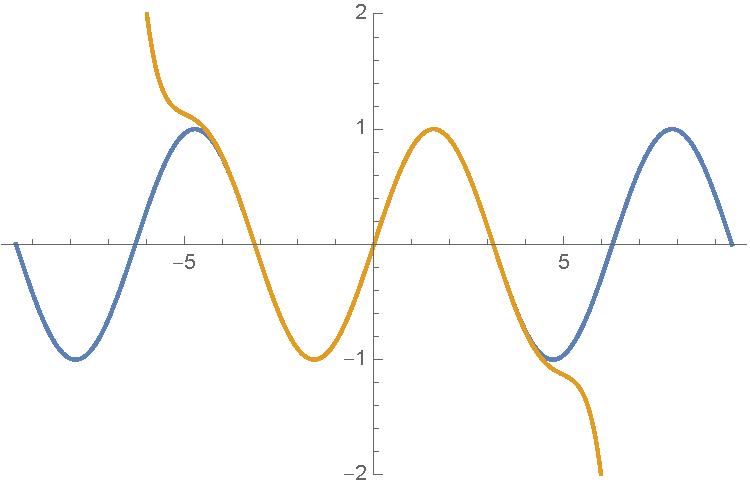
\includegraphics[scale=0.5]{./Figures/20180315-taylor-n11} %以pic.jpg的0.5倍大小输出
  \end{minipage}}
  \subfigure[$n=13$]{  %第二张子图
  \begin{minipage}{7cm}
    \centering  %子图居中
    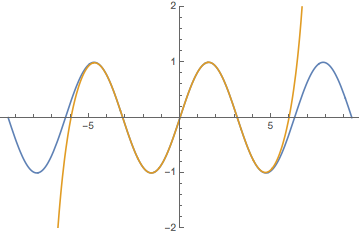
\includegraphics[scale=0.5]{./Figures/20180315-taylor-n13} %以pic.jpg的0.5倍大小输出
  \end{minipage}}
  \subfigure[$n=15$]{  %第二张子图
  \begin{minipage}{7cm}
    \centering  %子图居中
    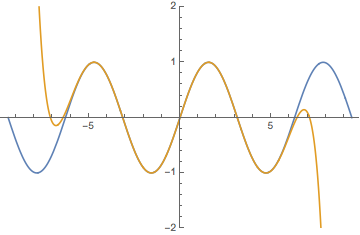
\includegraphics[scale=0.5]{./Figures/20180315-taylor-n15} %以pic.jpg的0.5倍大小输出
  \end{minipage}}
  \caption{麦克劳林级数的示例:对$\sin(x)$(蓝色曲线)沿着$x_{0}=0$作$n$阶泰勒级数展开(红色曲线)。} %大图名称
  \label{fig:maclaurin-series-example} %图片引用标记\end{figure}
%  \end{minipage}
\end{figure}

不难看出,$n$的值越大,近似的精度越高,如图\eqref{fig:maclaurin-series-example}所示。当$n \rightarrow \infty$时,近似是完全精确的。

当$a=0$时,泰勒级数变为沿着$x=a=0$的点作$n$阶泰勒展开,所生成的级数称麦克劳林级数(Maclaurin series)\index{Taylor-Maclaurin series \dotfill 麦克劳林级数}:
\begin{equation}
  \label{eq:taylor-maclaurin-series-def}
  f \left( x \right) = \frac{f(0)}{0!}
  + \frac{f^{'}(0)}{1!} \left( x  \right)
  + \frac{f^{''}(0)}{2!} \left( x \right)^{2}
  + \ldots
  + \frac{f^{(n)}(0)}{n!} \left( x \right)^{n}.
\end{equation}
\end{lemma}

\begin{lemma}[指数方程的麦克劳林级数(幂级数)]
  \label{lemma:exponential-maclaurin}
  现在设$f(x)= \exp x$。对应的麦克劳林级数展开由\eqref{eq:taylor-maclaurin-series-def}变为
\begin{equation}
  \label{eq:exponential-maclaurin-series-def}
  \begin{split}
    f \left( x \right) = \exp x & = \frac{f(0)}{0!}
    + \frac{f^{'}(0)}{1!} \left( x  \right)
    + \frac{f^{''}(0)}{2!} \left( x \right)^{2}
    + \ldots
    + \frac{f^{(n)}(0)}{n!} \left( x \right)^{n} \\
    & = 1 + \frac{x}{1!} + \frac{x^{2}}{2!} + \frac{x^{3}}{3!} + \frac{x^{4}}{4!} + \ldots \\
    & = \sum_{n=0}^{\infty} \frac{x^{n}}{n!}.
  \end{split}
\end{equation}
又称幂级数(power series)\index{power series \dotfill 幂级数}。
\end{lemma}

\begin{lemma}[正弦的麦克劳林级数]
  \label{lemma:sin-maclaurin-series}
  现在设$f(x) = \sin x$,对应的麦克劳林级数展开由\eqref{eq:taylor-maclaurin-series-def}变为
  \begin{equation}
    \label{eq:sin-cos-maclaurin-series}
    \begin{split}
      f \left( x \right) = \sin x & = \frac{f(0)}{0!}
      + \frac{f^{'}(0)}{1!} \left( x  \right)
      + \frac{f^{''}(0)}{2!} \left( x \right)^{2}
      + \ldots
      + \frac{f^{(n)}(0)}{n!} \left( x \right)^{n} \\
      & = \sin 0 + \frac{\cos 0}{1!} x
      + \frac{- \sin 0}{2!} x^{2}
      + \frac{- \cos 0}{3!} x^{3} + \ldots \\
      & = x - \frac{x^{3}}{3!} + \frac{x^{5}}{5!} - \frac{x^{7}}{7!} + \frac{x^{9}}{9!} - \ldots \\
      & = \sum_{n=0}^{\infty} \left( -1 \right)^{n} \frac{x^{2n+1}}{ \left( 2n + 1 \right)!}.
    \end{split}
  \end{equation}
\end{lemma}

\begin{lemma}[余弦的麦克劳林级数]
  \label{lemma:cos-maclaurin-series}
  类似地,若设$f(x)=\cos(x)$,有余弦的麦克劳林级数
  \begin{equation}
    \label{eq:cos-maclaurin-series}
  f(x) =   \cos x = 1 - \frac{x^{2}}{2!} + \frac{x^{4}}{4!} - \frac{x^{6}}{6!} + \frac{x^{8}}{8!} - \ldots = \sum_{n=0}^{\infty} \left( -1 \right)^{n} \frac{x^{2n}}{\left( 2n \right)!}.
  \end{equation}
\end{lemma}

\begin{lemma}[欧拉恒等式]
  \label{sec:euler-complex-identity}
  根据指数方程的麦克劳林级数(幂级数)引理(Lemma \ref{lemma:exponential-maclaurin}),将式\eqref{eq:exponential-maclaurin-series-def}中全部$x$都替换为$i x$,则有
  \begin{equation}
    \label{eq:euler-complex-identity}
    \begin{split}
      \exp \left[ i x \right] = \sum_{n=0}^{\infty} \frac{\left( i x \right)^{n}}{n!}
      & = 1 + \frac{\left( i \right) x}{1!}
      + \frac{\left( -1 \right) x^{2}}{2!}
      + \frac{\left( -i \right) x^{3}}{3!}
      + \frac{ x^{4}}{4!}
      + \ldots \\
      & = 1 + i \frac{x}{1!} - \frac{x^{2}}{2!}
      - i  \frac{x^{3}}{3!}
      + \frac{x^{4}}{4!}
      + i \frac{x^{5}}{5!}
      - \frac{x^{6}}{6!}
      - i \frac{x^{7}}{7!}
      + \ldots \\
      & =
      \left(
      1 - \frac{x^{2}}{2!} + \frac{x^{4}}{4!} - \frac{x^{6}}{6!} + \ldots
      \right)
      + i \left(
      x - \frac{x^{3}}{3!} + \frac{x^{5}}{5!} - \frac{x^{7}}{7!} + \ldots
      \right) \\
      & = \cos x + i \sin x.
    \end{split}
  \end{equation}
  又称欧拉恒等式(Euler identity)\index{Euler identity \dotfill 欧拉恒等式}。
\end{lemma}

\subsection{欧拉公式的作用}
\label{sec:euler-complex-uses}

欧拉公式、欧拉恒等式有什么用途?

\subsubsection{复数的坐标形式}
\label{sec:euler-coordinates}
一个复数(complex number)可以表示为一个时部和一个虚部相加的形式,例如对于复数$z$我们有
\begin{equation*}
\begin{split}
    z & = \Re(z) + i \Im(z) = x + i y, \quad x,y \in \mathbb{R}, \, i = \sqrt{-1}.
\end{split}
\end{equation*}

以实部为横轴,以虚部为纵轴,可以将$z$表示为复平面(complex plane)中的$(x,y)$点。我们常用模(magnitude)和角(angle),对应$\left\{ r, \theta \right\}$,来在复平面中表示$z$,如图\eqref{fig:euler-complex-plane}所示。

\begin{figure}[htbp]
  \caption{正弦函数的导数}
  \centering
  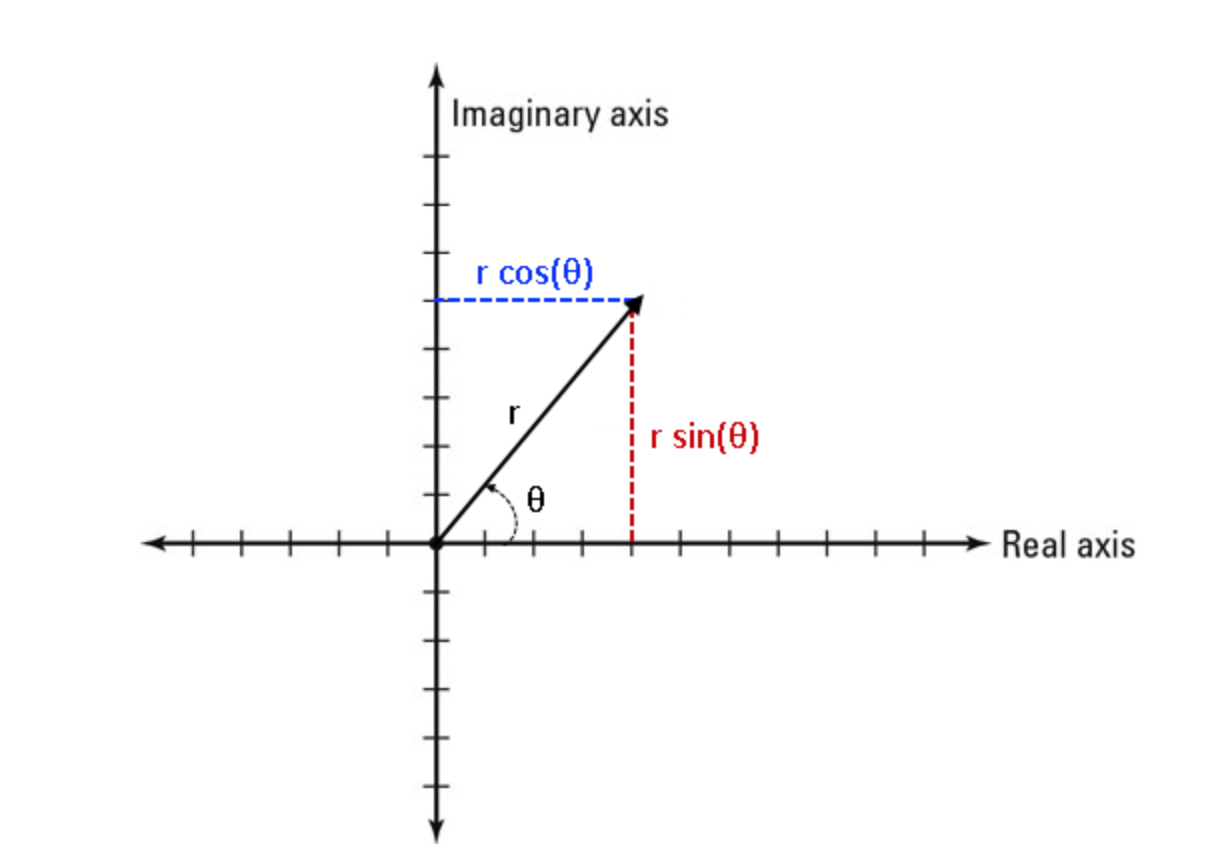
\includegraphics[width=8cm]{./Figures/20180401-complex-plane}
  \label{fig:euler-complex-plane}
%
%  \small{Source: PBOC.}
\end{figure}

由三角函数关系可得$x = r \cos \theta, \, y = r \sin \theta$,那么结合欧拉恒等式(Lemma \ref{sec:euler-complex-identity})可得
\begin{equation}
  \label{eq:euler-coordinates-complex-plane-z}
\begin{split}
    & z = x + i y = r \cos \theta + i r \sin \theta = r \left( \cos \theta + i \sin \theta \right) = r \exp \left( i \theta \right), \\
    & \hookrightarrow x + i y = r \exp \left( i \theta \right), \quad x = r \cos \theta, \, y = r \sin \theta,
\end{split}
\end{equation}
就是欧拉公式,将一个复数$z$写为关于夹角$\theta$和模$r$的三角方程

\subsubsection{复数的乘除}
\label{sec:euler-complex-multi-divid}
复数的乘除法如
\begin{equation*}
\begin{split}
  \left( a + b i \right) \left( c + d i \right)
  & = ac + a d i + b c i - b d = \left( ac - bd \right) + \left( ad + bc \right) i.
\end{split}
\end{equation*}

另一种算法时,假定要将两个指数方程相乘,满足
\begin{equation*}
  a \exp \left( i \theta \right) \cdot b \exp \left( i \theta \phi \right) = ab \exp \left[ i \left(\theta + \phi \right) \right],
\end{equation*}
即是说,两个复数相乘,就是分别将二者的模和夹角相乘。上式可以进一步写为
\begin{equation*}
  a \exp \left( i \theta \right) \cdot b \exp \left( i \theta \phi \right) = ab \left[ \cos \left( \theta + \phi \right) + i \sin \left( \theta + \phi \right) \right].
\end{equation*}

除法的操作类似。

\subsubsection{对复数的取幂}
\label{sec:euler-complex-exponentiation}

假设我们要计算$\left( a+bi \right)^{n}$的值。常见的简化方法之一是借助复数的形式
\begin{equation}
  \label{eq:euler-complex-exponentiation}
  \begin{split}
    \left( a+bi \right)^{n} & = \left[ r \exp
    \left(
    i \theta
    \right)
    \right]^{n}
    = r^{n} \exp \left( i \theta n \right)
    = r^{n} \left[ \cos \left( \theta n \right) + i \sin \left( \theta n \right) \right], \quad \forall \, n \in \mathbb{Z}_{+},
  \end{split}
\end{equation}
将一个复数的求幂运算(exponentiation)\index{exponentiation (complex analysis) \dotfill 取幂(复分析)}转换为幂指数的形式,又称棣莫弗定理(De Moivre Theorem)\index{De Moivre Theorem \dotfill 棣莫弗定理}。

前面介绍了如何将一个复数表示为幂指数形式,现在来看如何将一个实数表示为一个复数。已知欧拉公式\eqref{eq:euler-complex-def}
\begin{equation*}
  \exp \left[ i x \right] = \cos x + i \sin x,
\end{equation*}
将其中的$x$替换为$x \ln b$
\begin{equation*}
  \exp \left( i x \ln b \right) = \cos \left( x \ln b \right) + i \sin \left( x \ln b \right) = b^{i x},
\end{equation*}
那么,若对某个复数$y+ix$作幂,求$b^{y+ix}$的值,可计算如下
\begin{equation}
  \label{eq:euler-complex-exponentiation-xyi}
  b^{y+ix} = b^{y} \, b^{ix} = b^{y}
  \left[
  \cos \left( x \ln b \right) + i \sin \left( x \ln b \right)
  \right].
\end{equation}

举例:
\begin{equation*}
  5^{3+2i} = 5^{3} \, 5^{2i} = 5^{3} \left[ \cos \left( 2 \ln 5 \right) + i \sin \left( 2 \ln 5 \right) \right] \approx - 124.63 - 9.65 i.
\end{equation*}

\subsubsection{复值夹角}
\label{sec:euler-complex-angle-conjugate}
根据欧拉公式,可以进一步引出复值夹角(complex angle)\index{complex angle \dotfill 复值夹角}和三角方程的概念。先来看复值夹角。具体说来,前面我们所涉及到的正弦、余弦方程如$\sin(x)$,是对实数$x$的计算。如果要对一个复数求正弦余弦,该怎么操作?

对欧拉恒等式\eqref{eq:euler-complex-identity}作调整,用$-x$替代$x$,有
\begin{equation}
  \label{eq:euler-complex-identity-conjugate}
\begin{split}
  & \exp \left( i x \right) = \cos x + i \sin \left( x \right), \text{原方程}\\
  & \exp \left( - i x \right) = \cos x - i \sin \left( x \right) \text{复共轭},
\end{split}
\end{equation}
将一个复数的虚部变更符号(例如由正变为负),所组成的新的复数,称为原复数的复共轭(complex conjugate)\index{complex conjugate \dotfill 复共轭}。

现在对欧拉恒等式\eqref{eq:euler-complex-identity}及其复共轭\eqref{eq:euler-complex-identity-conjugate}相加和相减,得
\begin{align}
  \label{eq:euler-complex-identity-conjugate-plus}
  & \exp \left( i x \right) - \exp \left( - i x \right) = 2 i \sin x,  \Longleftrightarrow \sin x = \frac{\exp \left( i x \right) - \exp \left( - i x \right)}{2 i}, \\
  \label{eq:euler-complex-identity-conjugate-minus}
  & \exp \left( i x \right) + \exp \left( - i x \right) = 2 \cos x, \Longleftrightarrow \cos x = \frac{\exp \left( i x \right) + \exp \left( - i x \right)}{2},
\end{align}
即,我们得到了一组用指数(和虚数)表示的正弦、余弦方程。

调整\eqref{eq:euler-complex-identity-conjugate-plus}-  \eqref{eq:euler-complex-identity-conjugate-minus},用$ix$替换原式中的$x$,并且分子分母同时乘以$i$得
\begin{align}
  \label{eq:euler-complex-identity-conjugate-plus-i}
  & \sin \left( ix \right) = \frac{\exp \left( i^{2} x \right) - \exp \left( - i^{2} x \right)}{2 i^{2}} \frac{i}{i}
  = \frac{
  i \left[ \exp \left( x \right) - \exp \left( - x \right) \right]
  }{2} \equiv i \sinh x, \\
  \label{eq:euler-complex-identity-conjugate-minus-i}
  & \cos \left( ix \right) = \frac{\exp \left( i^{2} x \right) + \exp \left( - i^{2} x \right)}{2} \frac{i}{i} = \frac{
  \left[ \exp \left( x \right) + \exp \left( - x \right) \right]
  }{
  2
  } \equiv \cosh x,
\end{align}
其中$\sinh(x), \cosh(x)$分别称双曲线正弦方程和双曲线余弦方程(hyperbolic sine/cosine function)\index{hyperbolic function!sine \dotfill 双曲线正弦方程}\index{hyperbolic function!cosine \dotfill 双曲线余弦方程},如图  \ref{fig:sinh-cosh-function}。值得注意的是右图:任何虚数的余弦都是一个实数,原本的虚部消失不见。

\begin{figure}[htbp]
  \caption{双曲正弦/余弦方程,$x \in \left[ -3 \pi, 3 \pi\right]$}
  \centering
  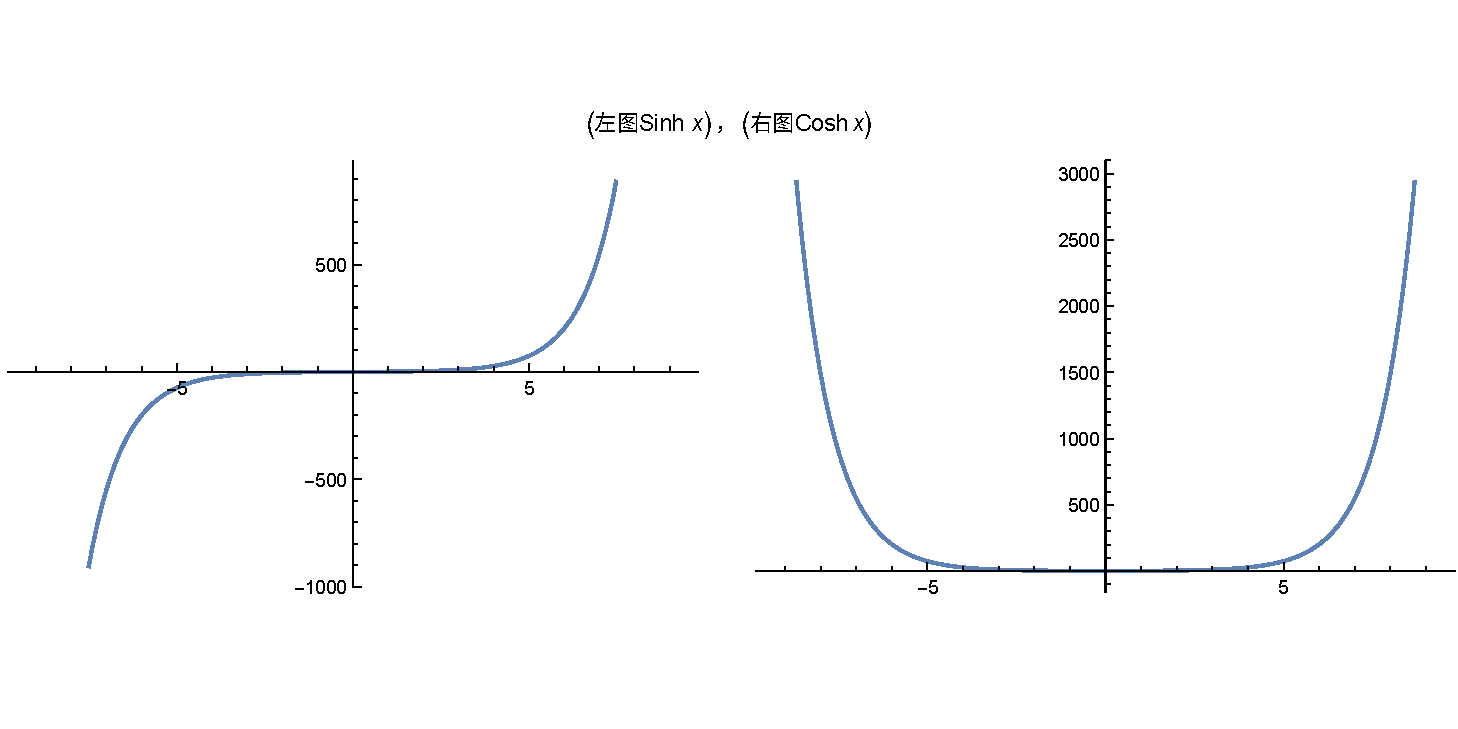
\includegraphics[width=12cm]{./Figures/20180401-sinh-cosh-x}
  \label{fig:sinh-cosh-function}
%
%  \small{Source: PBOC.}
\end{figure}

在此基础上,我们可以回答本节初提出的问题,如何计算一个复数的正弦/余弦,如$\sin \left( a + bi \right)$。
已知$\sin(a+b) = \sin a \cos b + \cos a \sin b$,并且$\sinh x, \cosh x$的定义如\eqref{eq:euler-complex-identity-conjugate-plus-i}-\eqref{eq:euler-complex-identity-conjugate-minus-i}所示。那么,用$bi$替换原式中的$b$,可得复数的正弦计算式
\begin{equation}
  \label{eq:complex-sin-abi}
\begin{split}
  \sin \left( a + b i \right) & = \sin a \cos \left( i b \right) + \cos a  \sin \left( i b \right) \\
  & = \sin a \cosh b + i \cos a \sinh b.
\end{split}
\end{equation}

余弦:$\cos \left( a + b \right) = \cos a \cos b - \sin a \sin b$。用$bi$替换$b$
\begin{equation}
  \label{eq:complex-cos-abi}
\begin{split}
  \cos \left( a + bi \right) & = \cos a \cos \left( ib\right) - \sin a \sin \left( i b \right) \\
  & = \cos a \cosh b - i \sin a \sinh b.
\end{split}
\end{equation}

举例:
\begin{equation*}
  \cos \left( 3 + 4 i \right)
  = \cos (3) \cosh (4) - i \sin (3) \sinh (4)
  \approx -27.03 + 3.85 i.
\end{equation*}
%\subsubsection{三角方程}
%三角方程(Trigonometry)

\section{高斯核方程}
\label{sec:kernel-analysis}

\subsection{高斯核}
\label{sec:kernel-gaussian}
%mchung teaching notes.
一个常见的高斯核方程(Gaussian kernel function)\index{kernel function!Gaussian \dotfill 高斯核方程},随着维度的不同,可以表示如下
\begin{align}
  \label{eq:kernel-gaussian-dim1}
  G^{(1)} \left( x ; \sigma \right) & = \frac{1}{\sqrt{2 \pi} \sigma}
  \exp \left( - \frac{x^{2}}{2 \sigma^{2}} \right), \\
  \label{eq:kernel-gaussian-dim2}
  G^{(2)} \left( x,y; \sigma \right)
  & = \frac{1}{2 \pi \sigma^{2}}
  \exp \left(  - \frac{x^{2} + y^{2}}{2 \sigma^{2}} \right), \\
  \vdots & \nonumber \\
  \label{eq:kernel-gaussian-dimN}
  G^{(N)} \left( \vec{x} ; \sigma \right)
  & = \frac{1}{\left(\sqrt{2 \pi} \sigma \right)^{N}}
  \exp \left(
  - \frac{
  \left| \vec{x} \right|^{2}
  }{
  2 \sigma^{2}
  }
  \right),
\end{align}
其中
\begin{itemize}
\item $\sigma > 0$表示高斯核的带宽(bandwidth),统计学中也将上式称为高斯概率密度方程(Gaussian probability density function)\index{probability density function (PDF)!Gaussian\dotfill 高斯概率密度方程}——对应地,称$\sigma$为标准差,$\sigma^{2}$为方差。
\item $\left\{ x \right\}$,$\left\{ x,y \right\}$分别表示1维和2维空间参数。$N$维空间参数往往用向量$\vec{x}$进行简化表示。
\item 空间参数和带宽参数之间的分号是常见的表达方式,提醒人们两者的含义不同。指数项中乘以$1/2$也是为了表述方便。
\end{itemize}

\subsection{标准化}
\label{sec:kernel-gaussian-normalization}
以1维高斯核方程\eqref{eq:kernel-gaussian-dim1}为例,前面的常数项$\frac{1}{\sqrt{2 \pi} \sigma}$是标准化常数,引入这个常数项是由于对$\exp \left( - \frac{x^{2}}{2 \sigma^{2}} \right)$沿着$x \in \left( - \infty, \infty \right)$求积,其值不等于$1$
\begin{equation*}
  \int_{-\infty}^{\infty} \exp \left( -
  \frac{x^{2}}{2 \sigma^{2}}
  \right) \mathrm{d} x = \sqrt{2 \pi} \sigma \neq 1.
\end{equation*}

在作标准化处理后,高斯核成为一个标准化的核方程,即满足
\begin{equation*}
  \int_{-\infty}^{\infty} G^{(1)} \left( x; \sigma \right)
  \, \mathrm{d} x = 1, \forall \, \sigma,
\end{equation*}
另一方面,增加带宽$\sigma$的值会显著降低$G^{(1)} \left( x ; \sigma \right)$的振幅(amplitude),例如$\sigma$取$0.3,1,2$三组不同的值,对应高斯方程\eqref{eq:kernel-gaussian-dim1}在$[-1.5\pi, 1.5\pi]$的形状,见图\ref{fig:gaussian-amplitude-sigma},图中取下下方阴影部分的面积均为$1$。
\begin{figure}[htbp]
  \caption{高斯核方程的振幅随带宽的增加而显著降低}
  \centering
  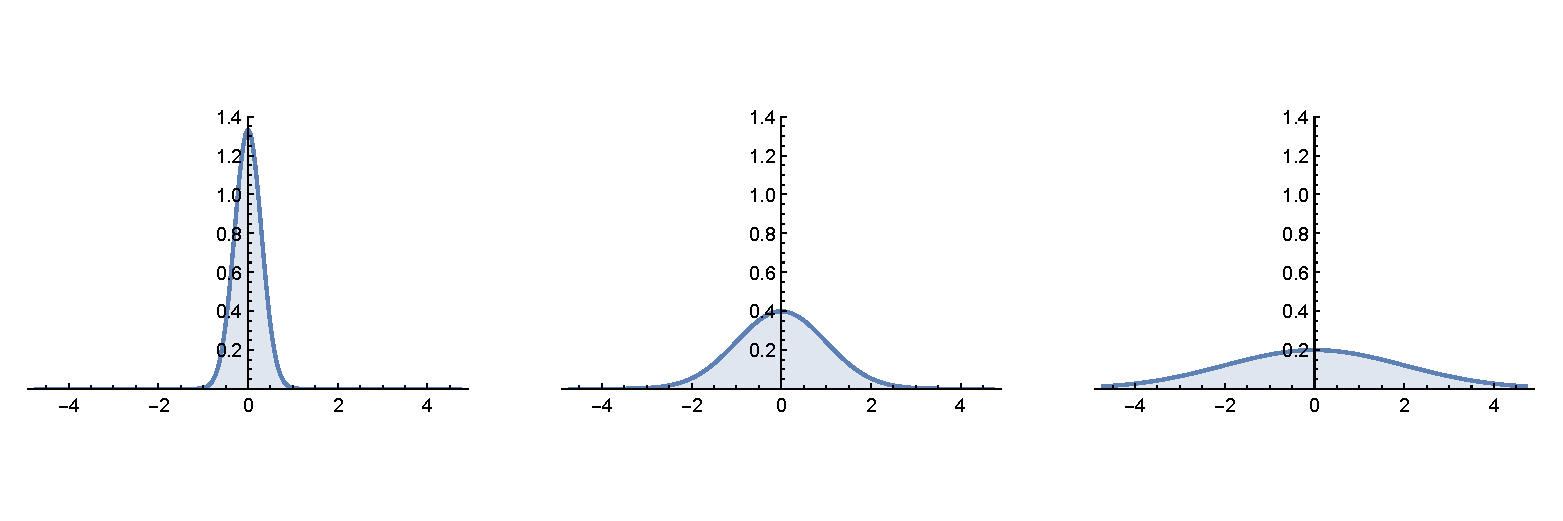
\includegraphics[width=12cm]{./Figures/20180404-gaussian-amplitude-sigma}
  \label{fig:gaussian-amplitude-sigma}
%
%  \small{Source: PBOC.}
\end{figure}

\subsection{瀑布特征}
\label{sec:kernel-gaussian-cascade}
将两个高斯核作卷积(convolution),可以得到一个新的高斯核方程,新方程具有与原方程相似的特性:
\begin{equation}
  \label{eq:kernel-gaussian-convolution}
  G_{1}\left( \vec{x_{1}}; \sigma_{1} \right)
  \, G_{2}\left( \vec{x_{2}}; \sigma_{2} \right)
  =  G_{new} \left( \vec{x} ; \sqrt{\sigma_{1}^{2} + \sigma_{2}^{2}} \right),
\end{equation}
我们称这种特性为自相似性(self-similarity)\index{self-similarity \dotfill 自相似性},高斯核方程就是这样一种自相似方程。

高斯方程的卷积是线性运算,那么高斯方程卷积的卷积也是线性运算,以此类推,这称为瀑布特性(cascade property)。

\subsection{带宽参数}
\label{sec:kernel-gaussian-bandwidth}
由于$\sigma_{1}^{2}+\sigma_{2}^{2}$较难直接计算,我们常常用$t \equiv 2 \sigma^{2}$的方式来做近似参数化处理。对于$N$维高斯核方程而言,有
\begin{equation*}
  G^{(N)} \left( \vec{x}; t\right) = \frac{1}{\left( \pi t \right)^{\frac{N}{2}}} \exp \left( - \frac{x^{2}}{t} \right).
\end{equation*}

如果$N=3$即向量$\vec{x}$中包括三组数据$\left\{x_{1},x_{2},x_{3}\right\}$,那么
\begin{equation*}
  \frac{\partial \mathcal{L}}{\partial t} = \sum_{i=1}^{3} \frac{\partial^{2} L}{\partial x_{i}^{2}},
\end{equation*}
即方差。


为了更好了解高斯核方程的自相似特征,我们引入一个无量纲(dimensionless)参数空间$\tilde{x} = \frac{x}{ \sqrt{2} \sigma}$来对$x$轴做"参数化"处理,对应的高斯核方程为
\begin{equation*}
\begin{split}
    G^{(N)} \left( \tilde{x}; \sigma \right) & = \frac{1}{\left( \sigma \sqrt{2 \pi} \right)^{N}} \exp \left( - \tilde{x}^{2} \right), \\
    G^{(N)} \left( \tilde{x}; t \right) & =
    \frac{1}{\left(\pi t\right)^{\frac{N}{2}}} \exp \left( - \tilde{x}^{2} \right),
\end{split}
\end{equation*}
两式等价。换句话说,沿着空间轴($x$轴)以$\sigma$的倍数为步长单位行走,其中所有的核方程都有相同的大小,又称带宽。

需要注意的是,带宽相同的高斯核,其振幅未必相同——这是由标准化计算流程所决定的。

在新的空间坐标系$\tilde{x}$中漫步,每一步的步长等于$\sqrt{2} \sigma$。对应地,我们称之为自然高斯核方程(natural) $G^{(N)} \left( \tilde{x} ; \sigma \right)$,对应的新坐标$\tilde{x} = \frac{x}{\sqrt{2} \sigma}$称为自然坐标。通过这种处理方法,可以从空间坐标系中去除方差$\sigma$,从而使得高斯核方程$G^{(N)}$彼此相似,区别只在于其(卷积$\tilde{x}$中的内方差)。

高斯核方程的值域是$\left( - \infty, \infty \right)$,但在现实应用中, $\left| x \right| > \sigma$的高斯核往往小到可以忽略不计。(如Mathematica计算$\sigma = 1, \, x = 5 \sigma$的高斯核)。

\subsection{狄拉克方程}
\label{sec:kernel-gaussian-dirac}
高斯核方程是一个半局部(semi-local)方程。之所以不是全局部的方程,是由于其卷积内部仍然存在着方差$\sigma$,从而使得空间里存在一个高斯加权范围(Gaussian weighted extend)。在下一节我们将提出一个通用方程来将其全局化,在此之前,本节先介绍一下狄拉克方程。

当将方差$\sigma$取其极限值$\lim \sigma \rightarrow 0$时,高斯核方程变成Delta方程的一种特殊形式,又称德尔塔-狄拉克方程(Delta-Dirac function)\index{Delta Dirac function \dotfill 狄拉克方程} $\delta(\cdot)$:
\begin{equation}
  \label{eq:kernel-gaussian-dirac-def}
\begin{split}
  \delta \left( \tilde{x} \right) \coloneqq \lim_{\sigma \rightarrow 0} G(\tilde{x}; \sigma) & = \lim_{\sigma \rightarrow 0} \frac{1}{\sqrt{2 \pi} \sigma}
  \exp \left( - \tilde{x}^{2} \right), \quad \tilde{x} = \frac{x}{\sqrt{2} \sigma} \\
  & = \lim_{\sigma \rightarrow 0} \frac{1}{\sqrt{2 \pi} \sigma} \exp \left( - \frac{x^{2}}{2 \sigma^{2}} \right) \\
  & = \begin{cases}
  \infty & x =0, \\
  0 & x \neq 0.
  \end{cases}
\end{split}
\end{equation}

在数学上,狄拉克方程$\delta \left( \cdot \right)$常称为取样方程。例如,对$f(x)$取$x=a$时的值,$a$是个常数。设$f(x)$在$x=a$处连续,可表示为如下求积形式
\begin{equation*}
  \int_{-\infty}^{\infty} \delta \left( x - a \right) \, f(x) \, \mathrm{d} x = f \left( a \right).
\end{equation*}

狄拉克方程的导数可定义如下
\begin{equation}
  \label{eq:kernel-gaussian-dirac-derivatives}
  \begin{split}
    \int_{-\infty}^{\infty} \delta^{'} (x) f(x) \, \mathrm{d} x & = - f^{'}(0),
    \\
    \int_{-\infty}^{\infty} \delta^{''} (x) f(x) \, \mathrm{d} x & = - f^{''}(0).
  \end{split}
\end{equation}

将全部$\left( -\infty, x \right]$区间中的高斯核加总,称为累积高斯方程(culmulative Gaussian kernel function)\index{kernel function!Gaussian, culmulative \dotfill 累积高斯核方程},又称误差方程(error function)\index{error function \dotfill 误差方程}
\begin{equation}
  \label{eq:kernel-gaussian-culmulative}
  err \left( x; \sigma \right) \coloneqq \int_{0}^{x} \frac{1}{\sqrt{2 \pi} \sigma} \exp \left( - \frac{y^{2}}{2 \sigma^{2}}\right) \, \mathrm{d} y,
\end{equation}
在Mathematica中运行程序,返回值$\frac{1}{2} Erf\left[ \frac{x}{\sqrt{2 \pi} \sigma} \right]$。$Erf[]$是Mathematica内建的高斯误差计算方程,前面乘以1/2是因为求积区间只是$[0,x]$,是$[-x,x]$的一半。

现在逐渐减少$\sigma$的值,$1.0 \rightarrow 0.1$。不难看出,随着$\sigma$越来越接近于$0$,在$x=0$附近就越会出现较大的跃动,如图\eqref{fig:gaussian-kernel-sigma-value}。
\begin{figure}[htbp]
  \caption{误差方程(累积高斯方程)随$\sigma$值的变化}
  \centering
  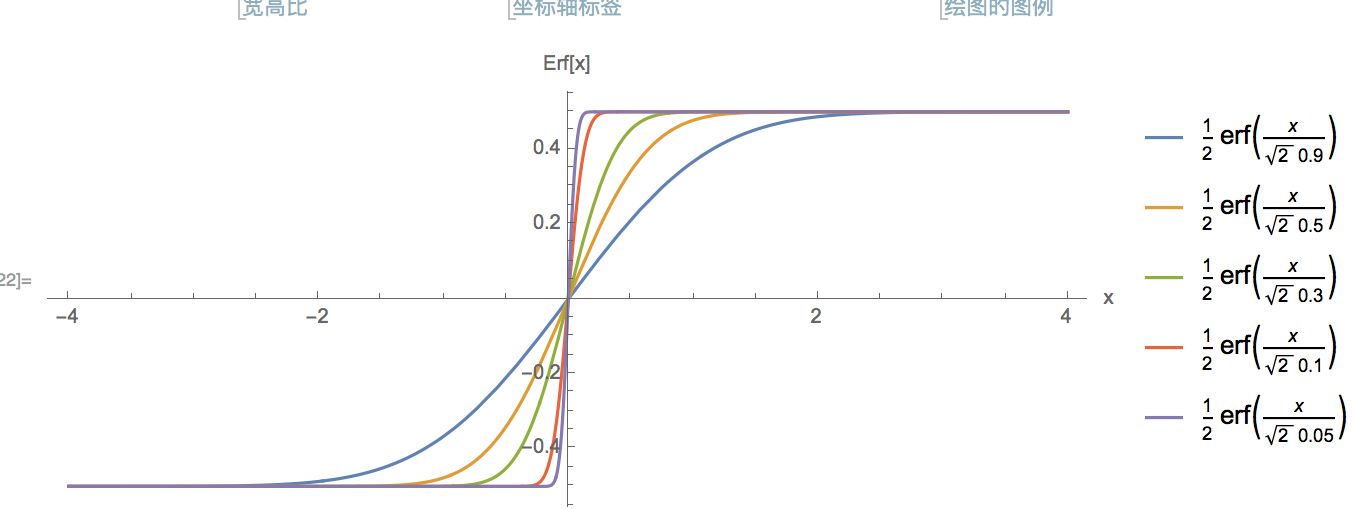
\includegraphics[width=12cm]{./Figures/20180405-gaussian-sigma-value}
  \label{fig:gaussian-kernel-sigma-value}
%
%  \small{Source: PBOC.}
\end{figure}

取$\lim \sigma \rightarrow 0$,内部方差趋近于$0$,此时的误差方程我们成为Heaviside 单位阶跃方程(unit step function)\index{unit step function \dotfill 单位阶跃方程},又称黑维塞方程(Heaviside function)\index{Heaviside function \dotfill 黑维塞方程}。黑维塞方程的导数也是一个狄拉克方程。

\begin{figure}[htbp]
  \caption{黑维塞方程(单位阶跃方程)}
  \centering
  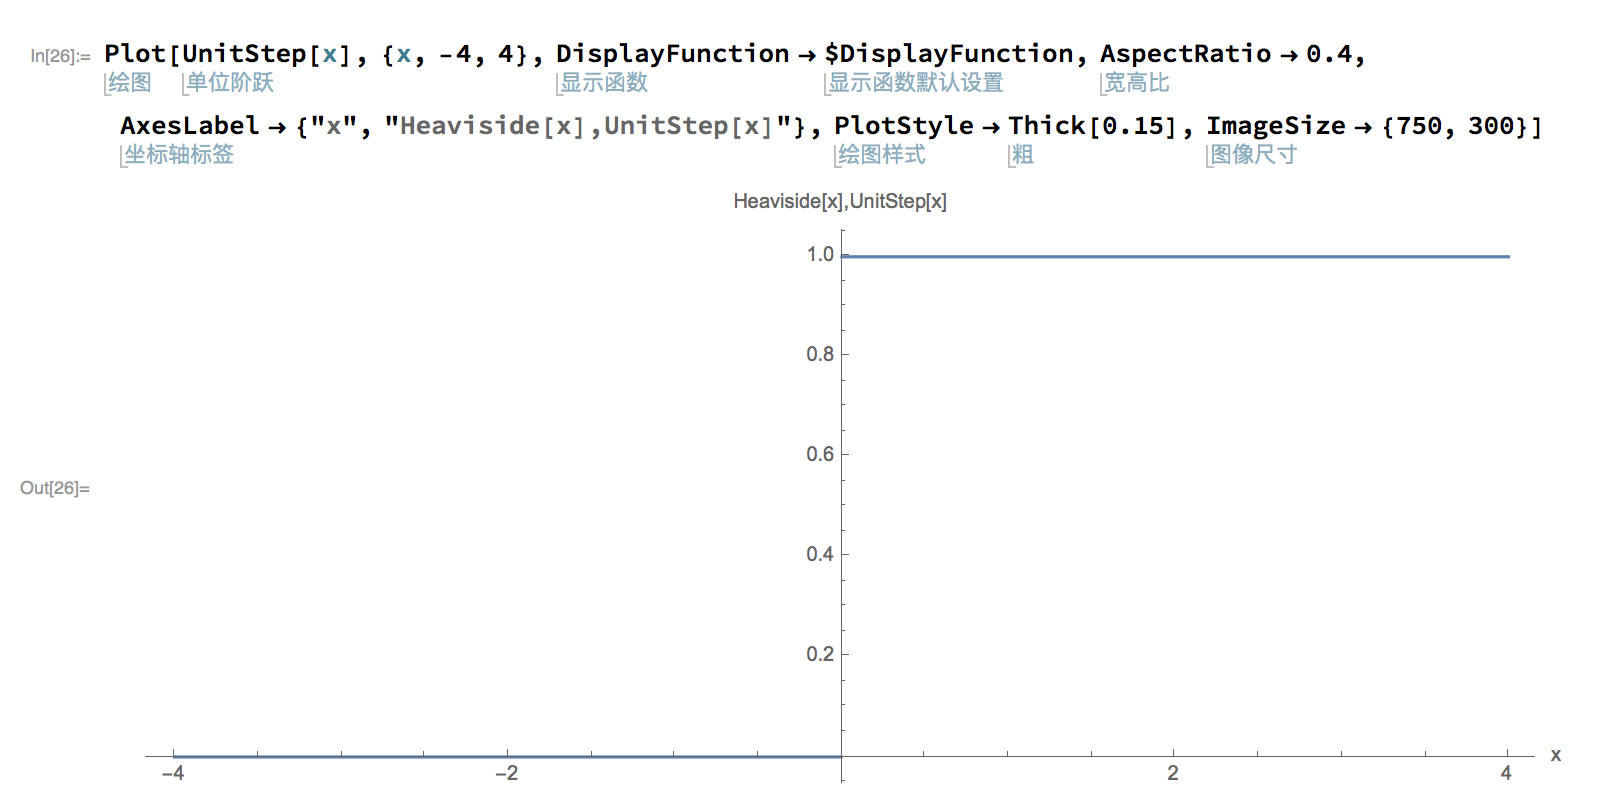
\includegraphics[width=12cm]{./Figures/20180405-heaviside-unit-step-function}
  \label{fig:heaviside-unite-step-function}
%
%  \small{Source: PBOC.}
\end{figure}

\subsection{高斯核和二项式系数的关系}
\label{sec:kernel-gaussian-binomial}
高斯核方程也常用于多项式的幂,如
\begin{equation*}
  \begin{split}
    (x+y)^{20}
    =& x^{20}+20 x^{19} y+190 x^{18} y^2+1140 x^{17} y^3+4845 x^{16} y^4+15504 x^{15} y^5+38760 x^{14} y^6+77520 x^{13} y^7\\
    &+125970 x^{12} y^8+167960 x^{11} y^9+184756 x^{10}
   y^{10}+167960 x^9 y^{11}+125970 x^8 y^{12}+77520 x^7 y^{13}\\
   &+38760 x^6 y^{14}+15504 x^5 y^{15}+4845 x^4 y^{16}+1140 x^3 y^{17}+190 x^2 y^{18}+20 x y^{19}+y^{20},
  \end{split}
\end{equation*}
RHS中各项前的系数,称二项式系数(binomial coefficients)\index{binomial coefficients \dotfill 二项式系数}。二项式系数常常表示为
\begin{equation*}
  \begin{pmatrix}
    n \\ m
  \end{pmatrix}
\end{equation*}
的形式,在Mathematica中用$Binomial[n,m]$来生成,见图\ref{fig:binomial-coefficients},从左到右分别是一维和二维二项式系数的示例。

\begin{figure}[htbp]
  \caption{二项式系数}
  \centering
  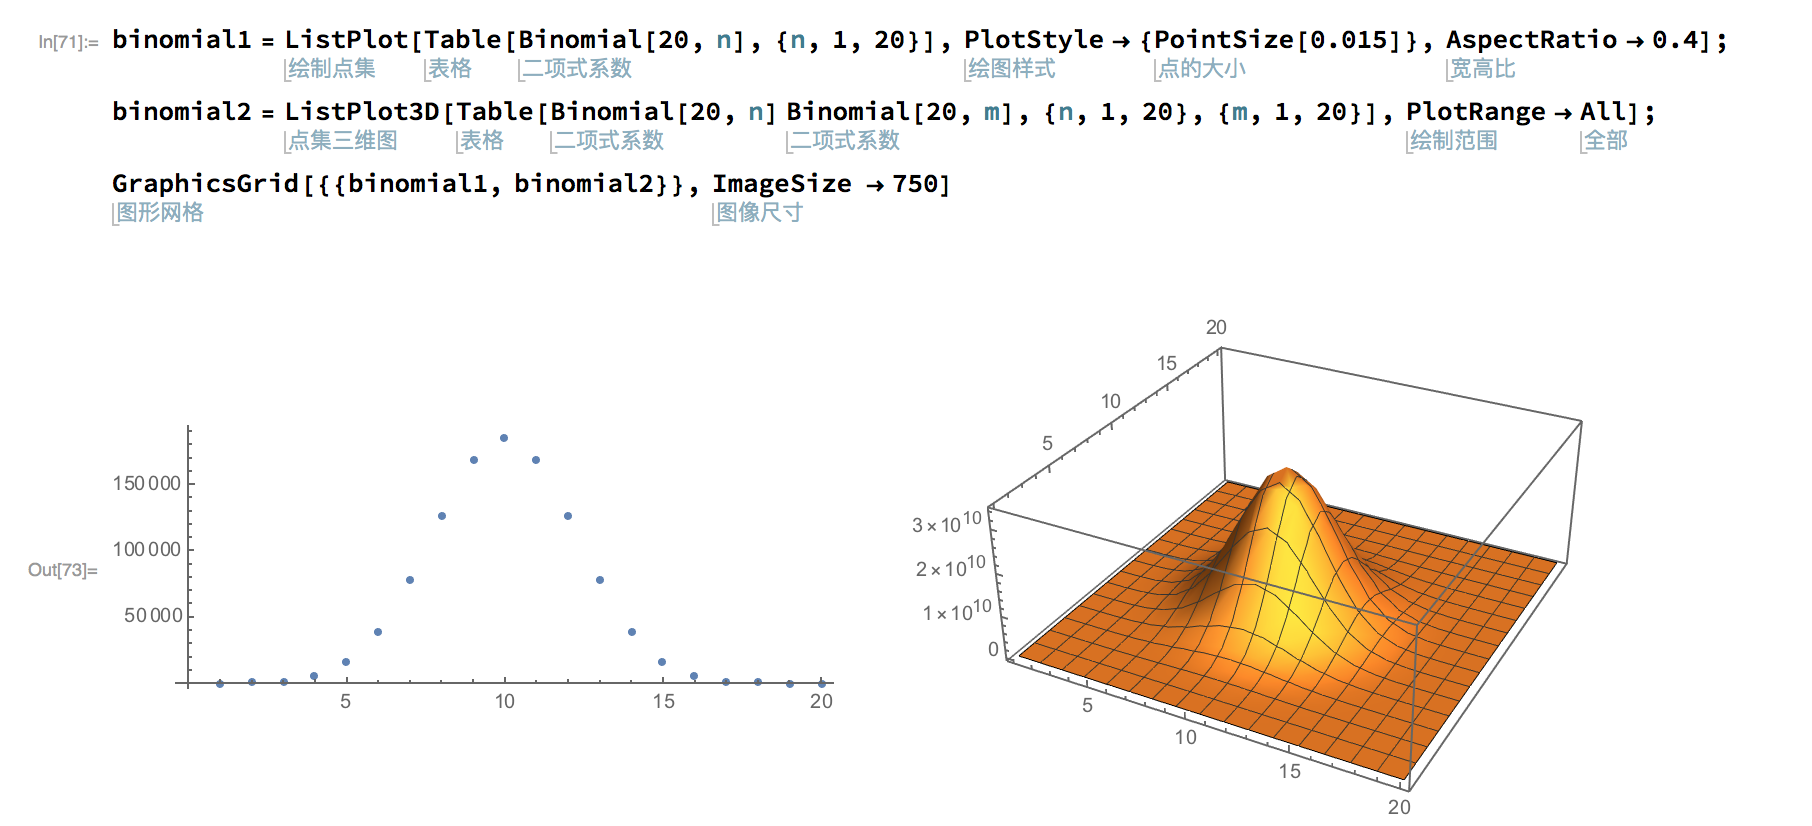
\includegraphics[width=12cm]{./Figures/20180405-binomial-coefficients}
  \label{fig:binomial-coefficients}
%
%  \small{Source: PBOC.}
\end{figure}


\subsection{中心极限定理}
\label{sec:kernel-gaussian-central-limit-theorem}
设两个块方程$f(x), \, g(x)$,均由两个黑维塞方程相加而得,定义为
\begin{equation*}
  \begin{split}
    f(x) & \coloneqq UniteStep \left( \frac{1}{2} + x \right) + UniteStep \left( \frac{1}{2} + - \right) -1, \\
     g(x) & \coloneqq UniteStep \left( \frac{1}{2} + x \right) - UniteStep \left( \frac{1}{2} + - \right) -1, \\
  \end{split}
\end{equation*}
见图\eqref{fig:convolution-fg},不难看出,两个黑维塞方程相加减还是黑维塞方程。

\begin{figure}[htbp]
  \caption{黑维塞方程相加减}
  \centering
  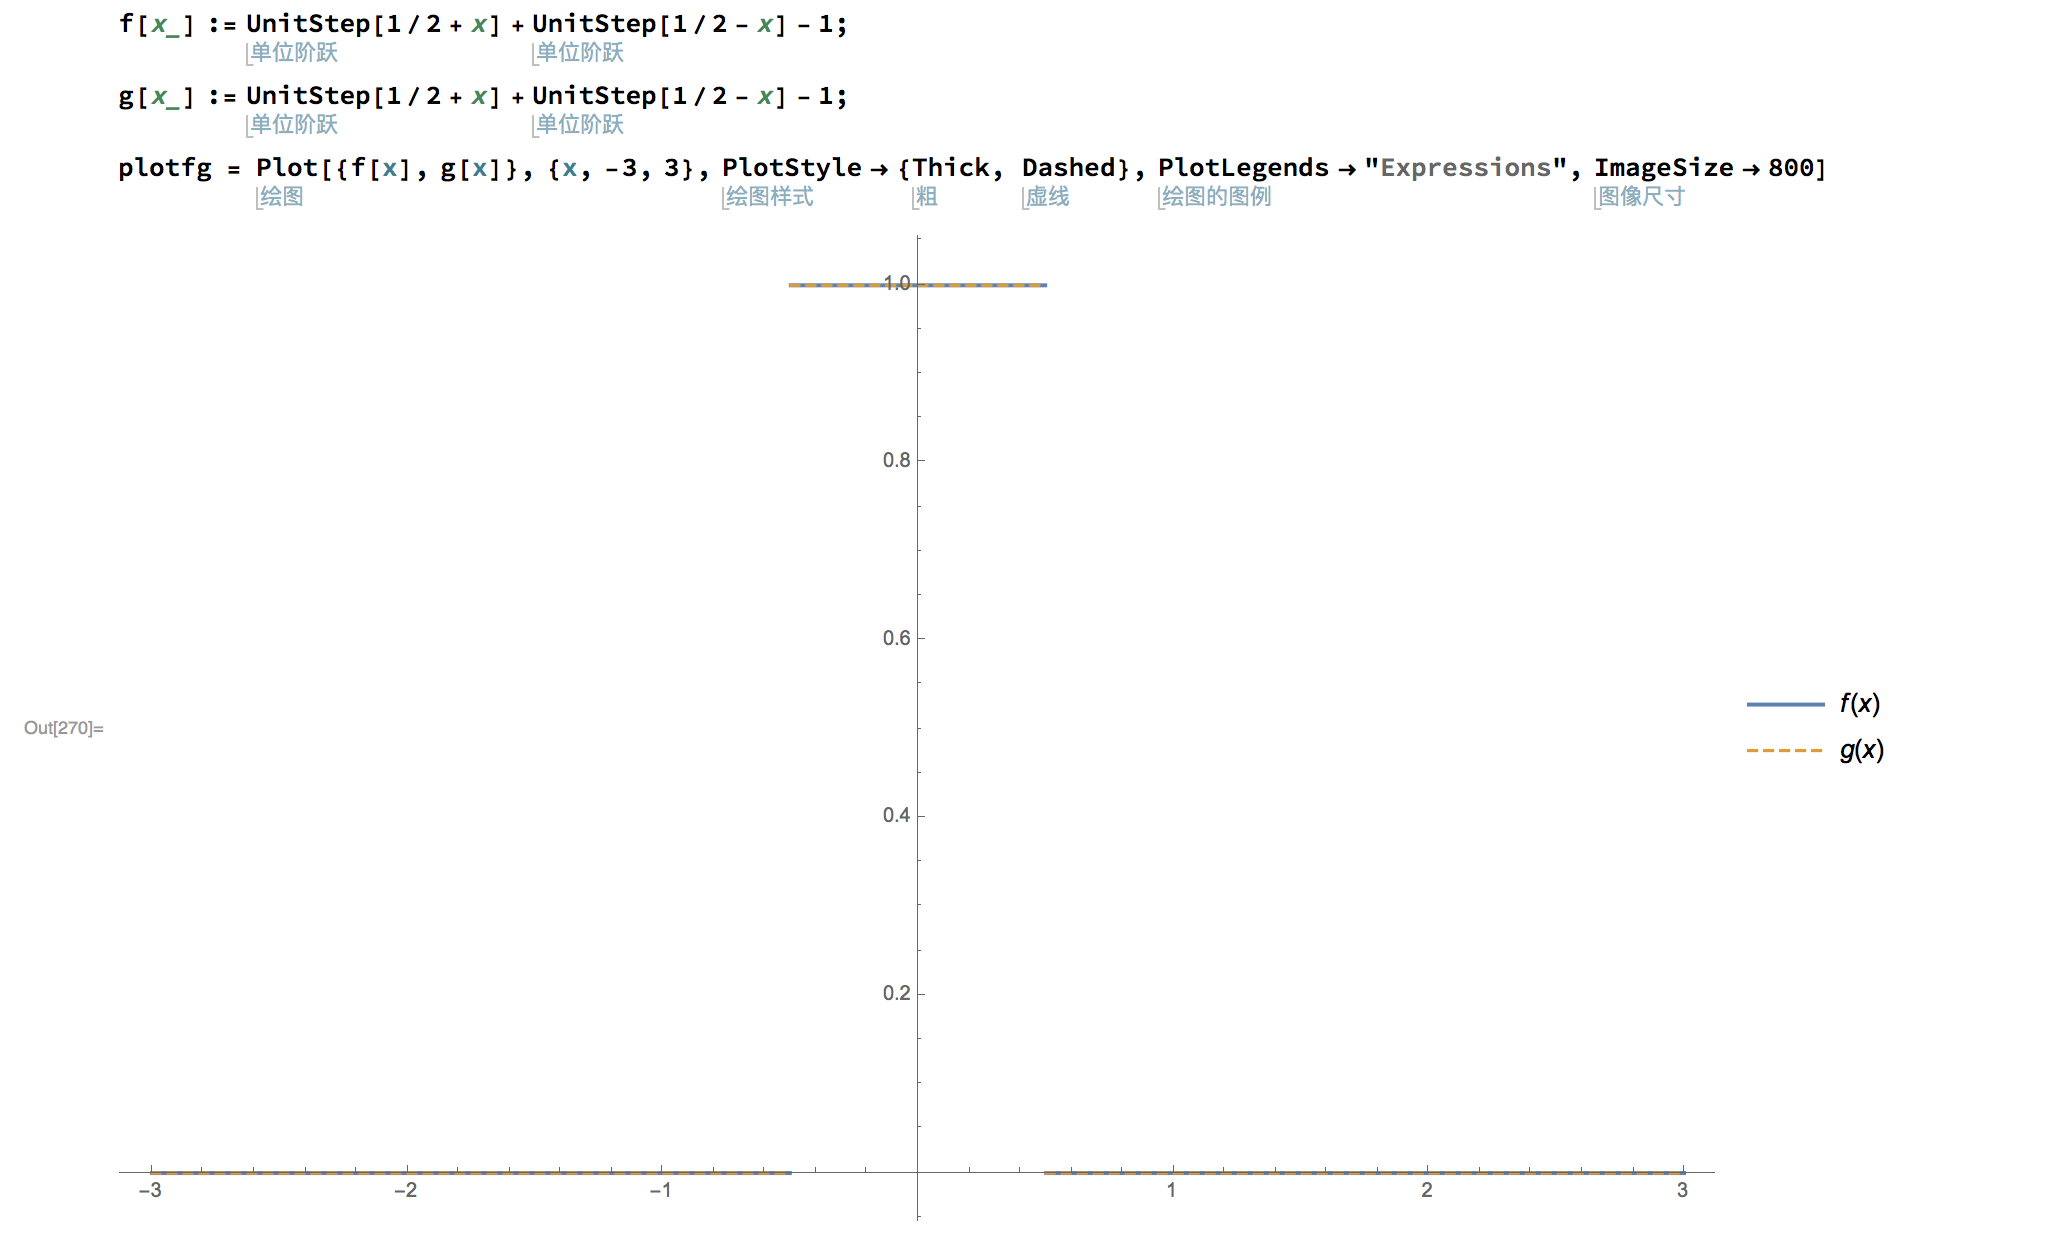
\includegraphics[width=10cm]{./Figures/20180405-convolution-fg}
  \label{fig:convolution-fg}
%
%  \small{Source: PBOC.}
\end{figure}

现在求卷积$\langle f(x), \, g (x) \rangle$
\begin{equation*}
  \langle f(x), \, g (x) \rangle =
  \int_{-\infty}^{\infty} f \left( x \right) \, g \left( x - x_{1} \right) \, \mathrm{d} x,
\end{equation*}
见图\ref{fig:convolution-fg-1},不难看出,两个块方程的卷积是一个三角方程。
\begin{figure}[htbp]
  \caption{两个块方程的卷积是一个三角方程}
  \centering
  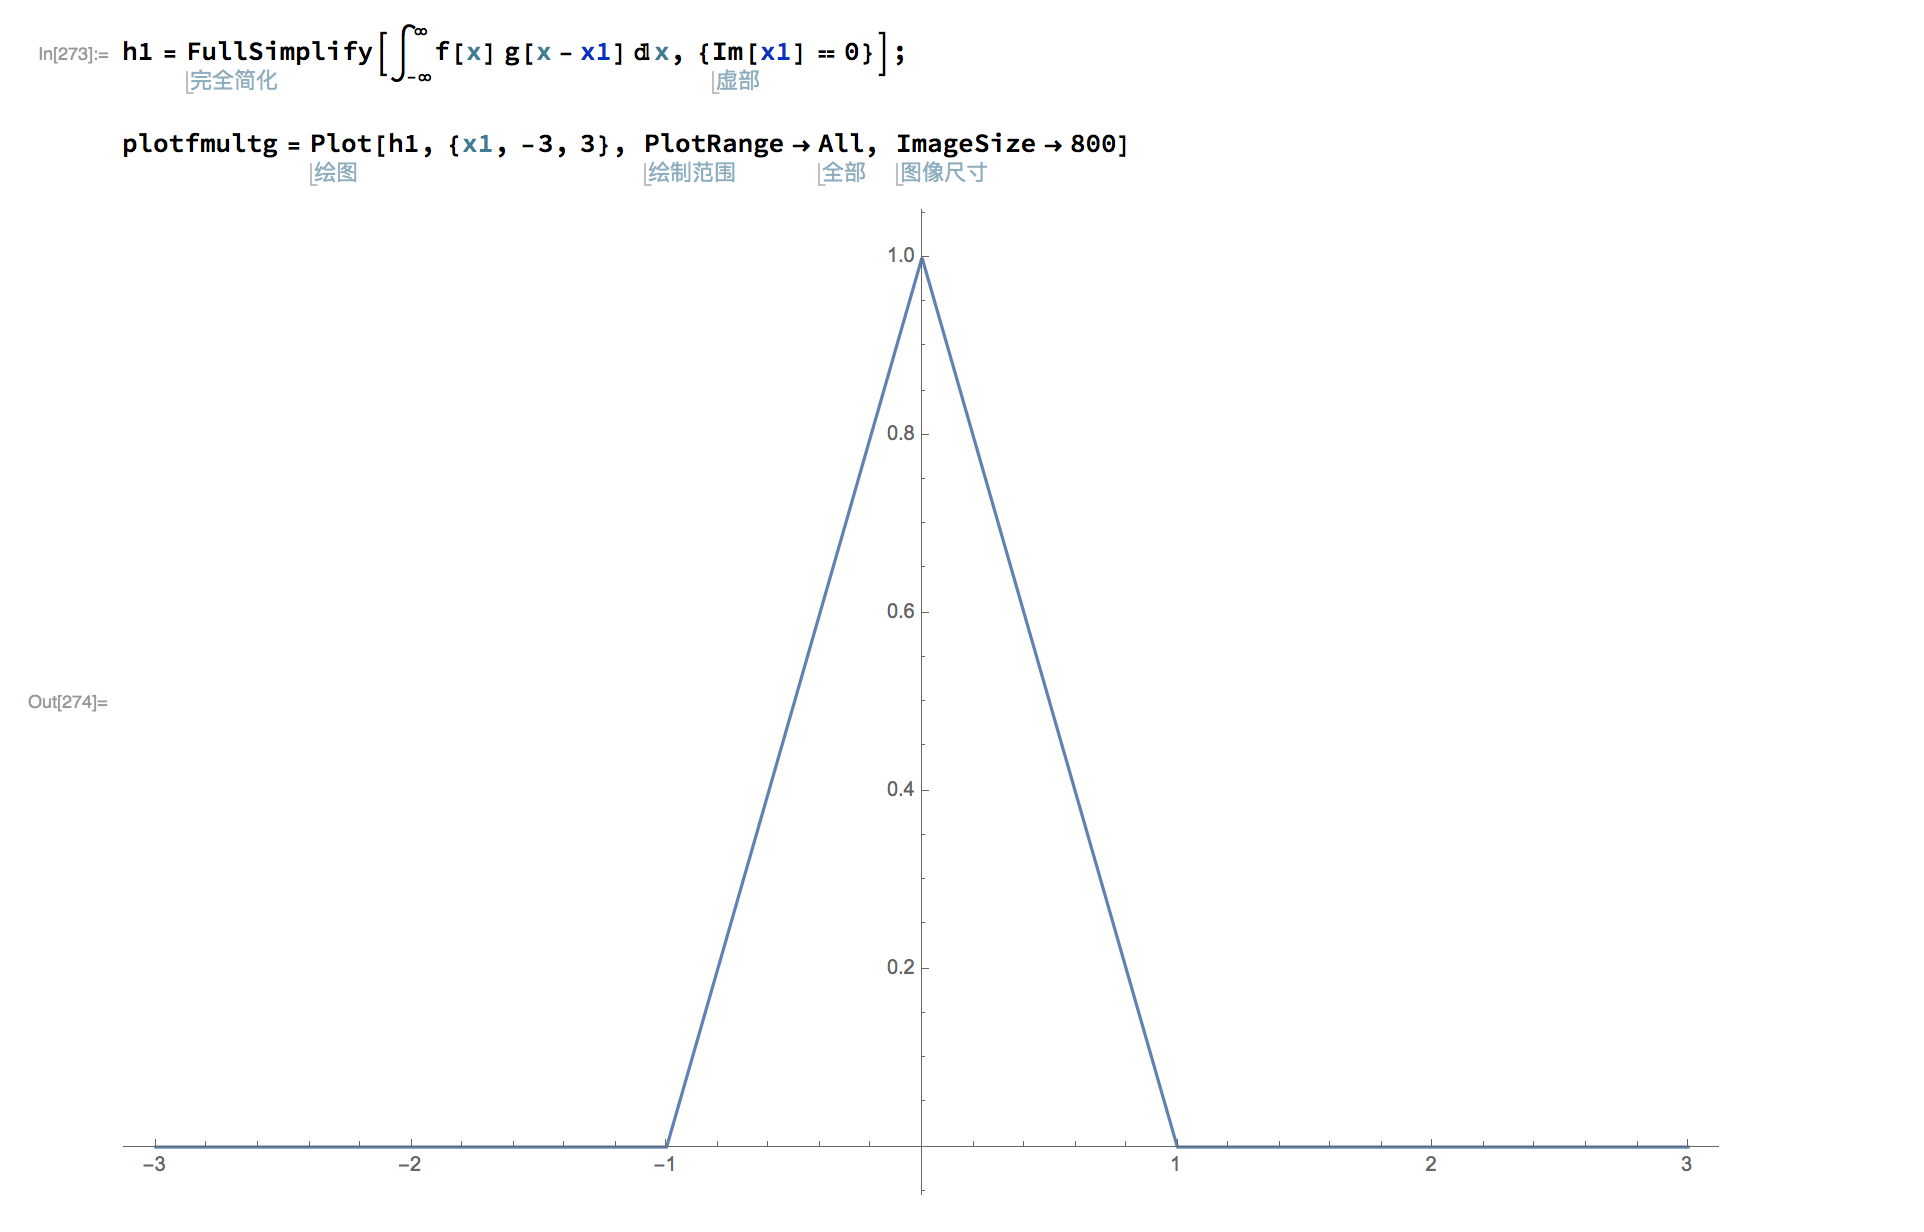
\includegraphics[width=10cm]{./Figures/20180405-convolution-fg-1}
  \label{fig:convolution-fg-1}
%
%  \small{Source: PBOC.}
\end{figure}

若对卷积再做一次卷积$  \langle \langle f(x), \, g (x) \rangle, \, g (x) \rangle$
\begin{equation*}
  \Big\langle \langle f(x), \, g (x) \rangle, \, g (x) \Big\rangle
  = \int_{-\infty}^{\infty}
  \left\{
  \int_{-\infty}^{\infty} f \left( x \right) \, g \left( x - x_{1} \right) \, \mathrm{d} x
  \right\}
  \, g \left( x - x_{1} \right) \, \mathrm{d} x,
\end{equation*}
如图\ref{fig:convolution-fg-2},可见对块方程,用它和自身再做一次卷积,二次卷积的结果看起来就很接近一个高斯核方程了。
\begin{figure}[htbp]
  \caption{两个块方程卷积的卷积接近一个高斯分布}
  \centering
  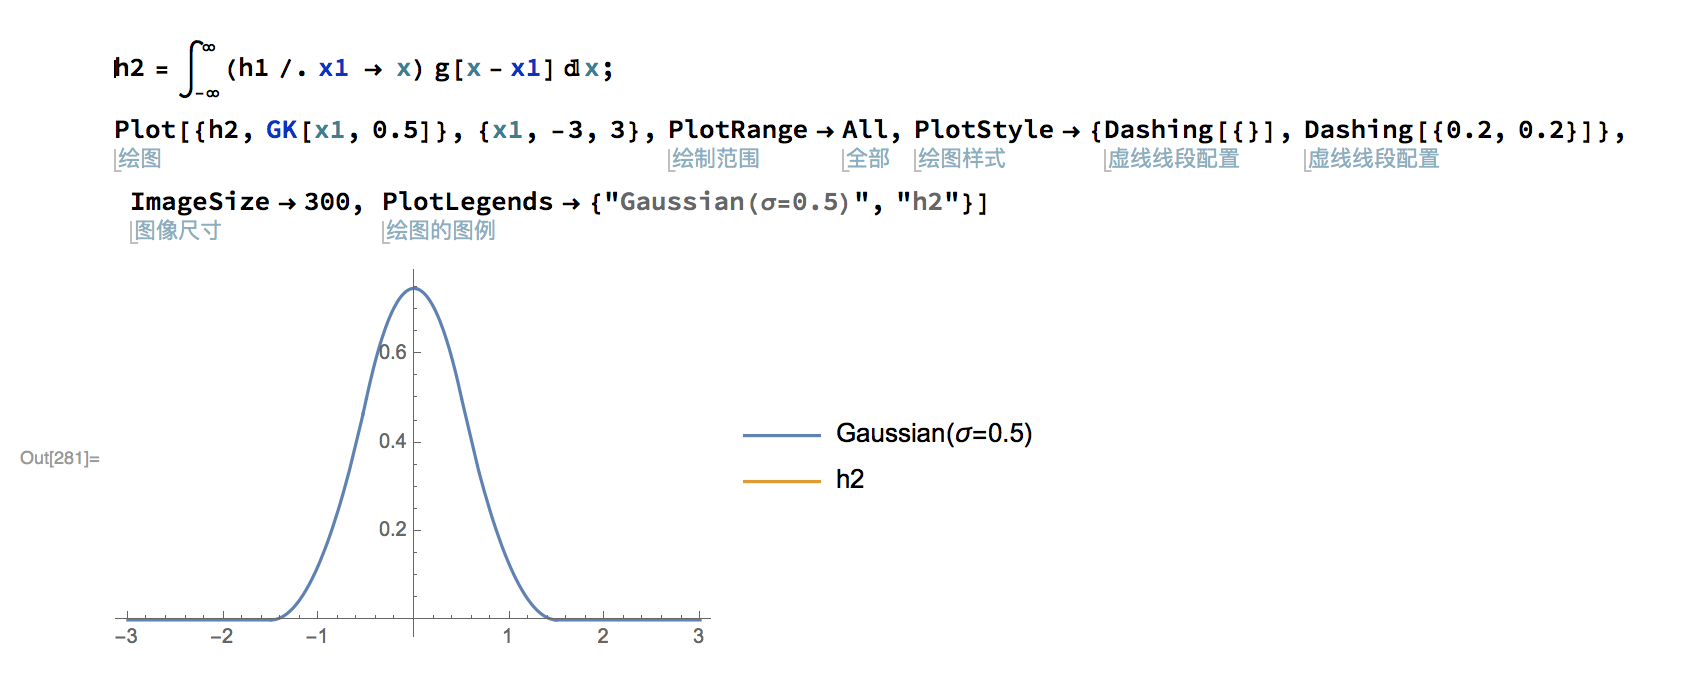
\includegraphics[width=10cm]{./Figures/20180405-convolution-fg-2}
  \label{fig:convolution-fg-2}
%
%  \small{Source: PBOC.}
\end{figure}

随着我们进一步作第$3,4,\ldots,N$次卷积,$N \rightarrow \infty$时的结果就是一个高斯核方程。这便是中心极限定理(central limit theorem, CLT)\index{central limit theorem (CLT) \dotfill 中心极限定理}。

\subsection{各向同性和各向异性}
\label{sec:kernel-gaussian-isotropy-anisotropy}
前面提到的高斯方程都具有各项同性(isotropy)\index{isotropy}的特征,意味着如果方差相同,那么方程向各个方向的变化是相同的。以2维高斯方程\eqref{eq:kernel-gaussian-dim2}为例,设$\sigma =1$,则(讨论1维没有意义)
\begin{equation*}
  \begin{split}
    \frac{\partial}{\partial x} G^{(2)} \left( x,y;1 \right)
    & = \frac{x}{2 \pi}
    \exp \left(  - \frac{x^{2} + y^{2}}{2} \right),\\
    \frac{\partial}{\partial y} G^{(2)} \left( x,y;1 \right)
    & = \frac{y}{2 \pi}
    \exp \left(  - \frac{x^{2} + y^{2}}{2} \right),
  \end{split}
\end{equation*}
高斯核对$x,y$的偏导表现为图\ref{fig:gaussian-isotropy-2d}中的箭头,沿着各个方向的变化幅度相同,呈圆形;每个箭头所指的方向,构成一个梯度向量(gradient vector)。
\begin{figure}[htbp]
  \caption{2维空间中高斯方程的各项同性}
  \centering
  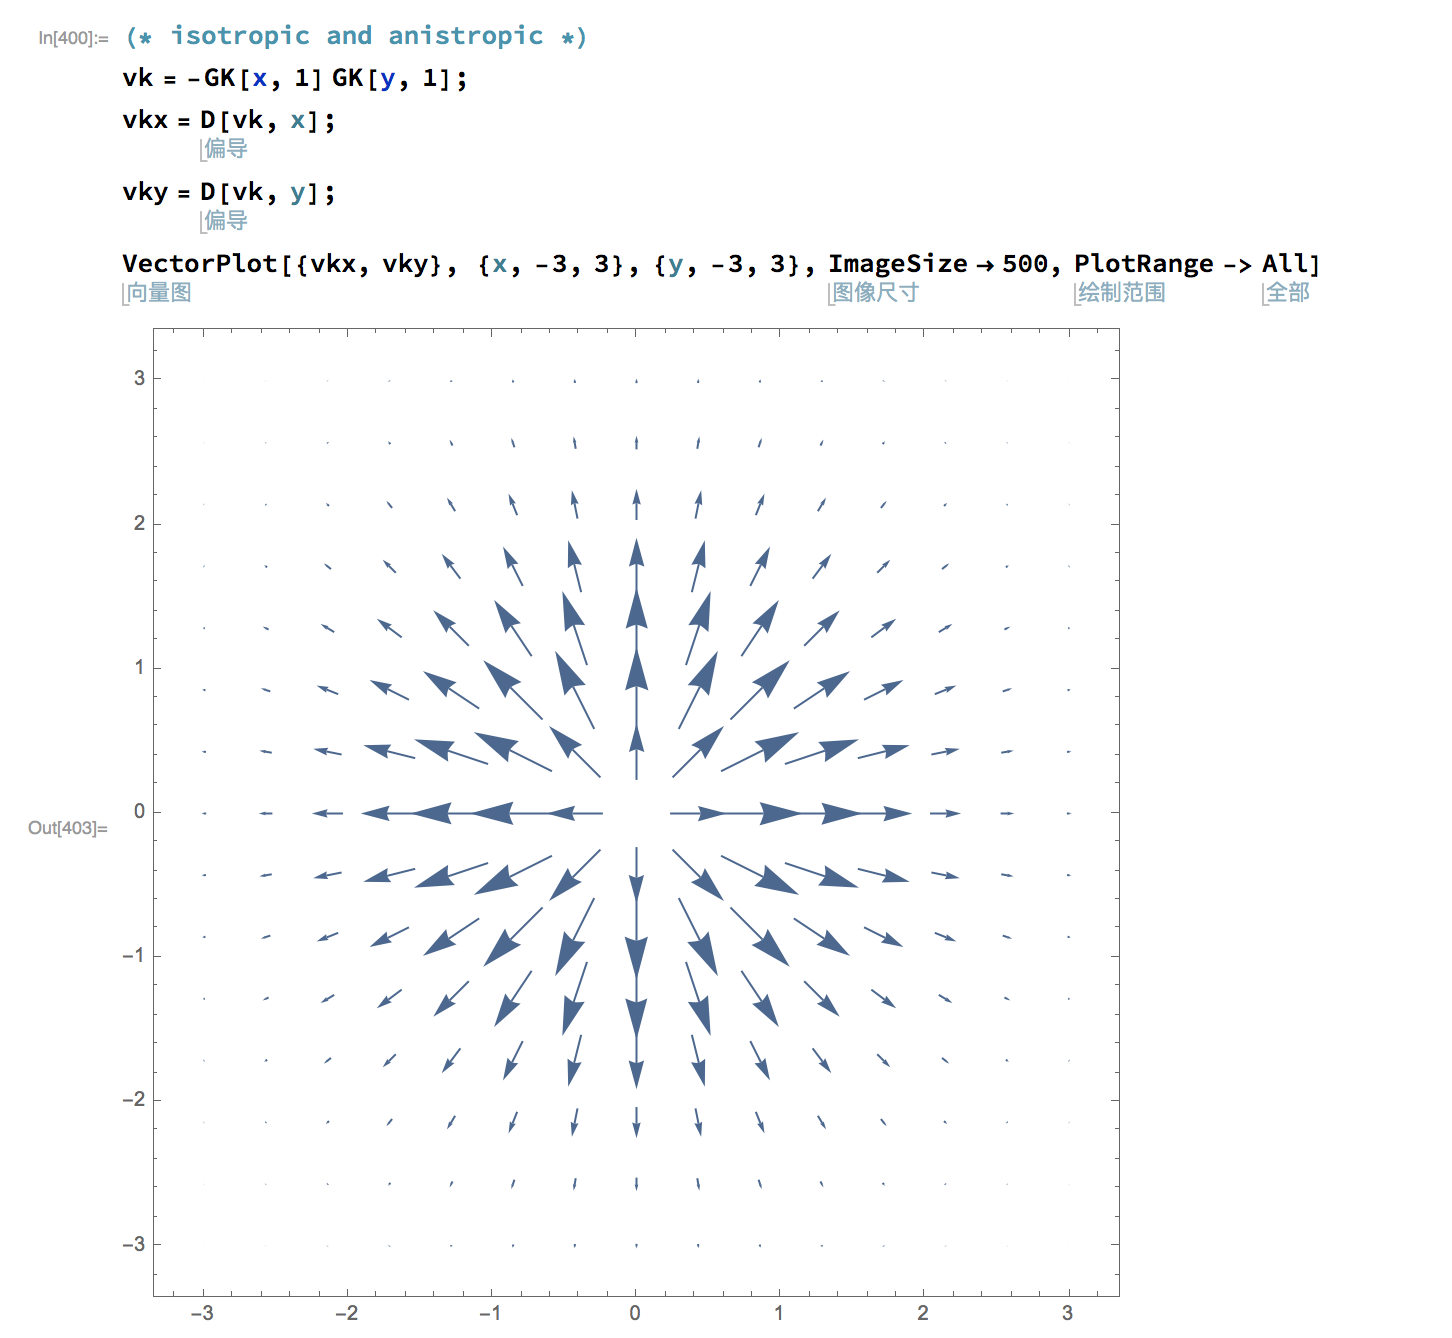
\includegraphics[width=10cm]{./Figures/20180405-isotropy}
  \label{fig:gaussian-isotropy-2d}
%
%  \small{Source: PBOC.}
\end{figure}
类似地,保持方差不变,3维高斯方程的导数表现为一个球形。

另一方面,如果方差不同,那么$N>1$维高斯方程在各个维度中的变化不同,我们称之为各向异性(anisotropy)\index{anistropy \dotfill 各向异性},如图\ref{fig:gaussian-anisotropy-2d}。
\begin{figure}[htbp]
  \caption{2维空间中高斯方程的各项异性}
  \centering
  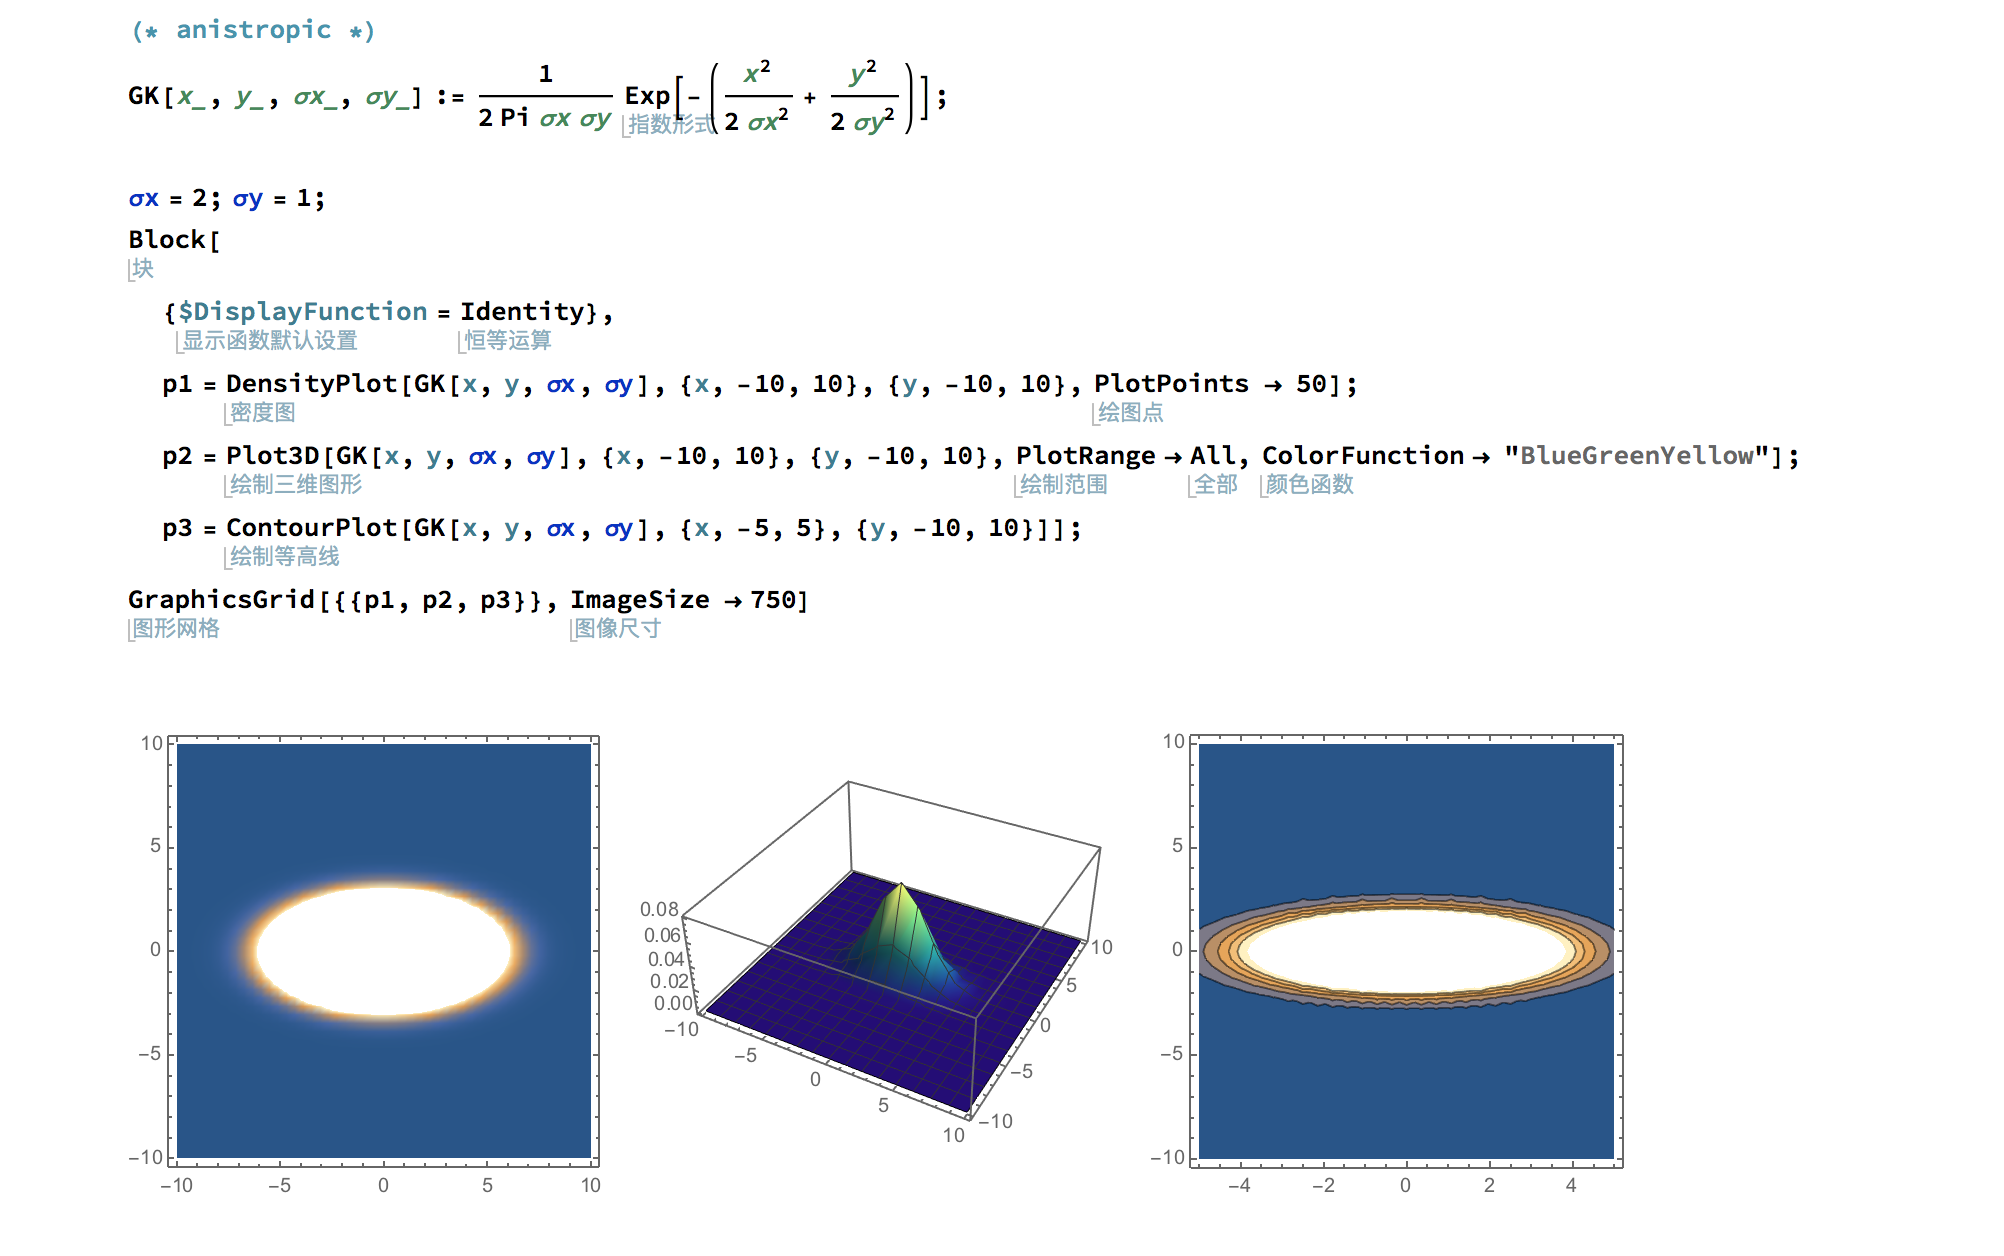
\includegraphics[width=12cm]{./Figures/20180405-anisotropy}
  \label{fig:gaussian-anisotropy-2d}
%
%  \small{Source: PBOC.}
\end{figure}

\subsubsection{高斯核方程的傅里叶变换}
\label{sec:gaussian-kernel-fourier}
实际研究中常常将实值域中的求积问题变换为傅里叶域中来计算,因为后者更方便。更多傅里叶变换的介绍见第\ref{sec:fourier-analysis}节。

傅里叶变换$\mathcal{F}$常用来表示,对应基方程$\exp \left( i \omega x \right)$,常用的傅里叶变换以及逆傅里叶变换$\mathcal{F}^{-1}$可表示为
\begin{align}
  \label{eq:gaussian-kernel-fourier-trans}
  \mathcal{F} \left( f(x) \right) & = F \left( \omega \right)
  \frac{1}{2 \sqrt{\pi}} \int_{-\infty}^{\infty} f(x) \, \exp \left( i \omega x \right) \, \mathrm{d} x = \frac{1}{2 \sqrt{\pi}} \exp \left( - \frac{1}{2} \sigma^{2} \omega^{2} \right), \\
  \mathcal{F}^{-1} \left( F \left( \omega \right) \right)
  & = \frac{1}{2 \sqrt{\pi}} \int_{-\infty}^{\infty} F \left( \omega \right) \exp \left( - i \omega x \right) d \omega.
\end{align}
在Mathematica中,可以自己写出$\mathcal{F}, \, \mathcal{F}^{-1}$的程序,或者用自带程序,见图\ref{fig:fourier-transform-mma.png}。
\begin{figure}[htbp]
  \caption{傅里叶变换、逆傅里叶变换的Mathematica程序}
  \centering
  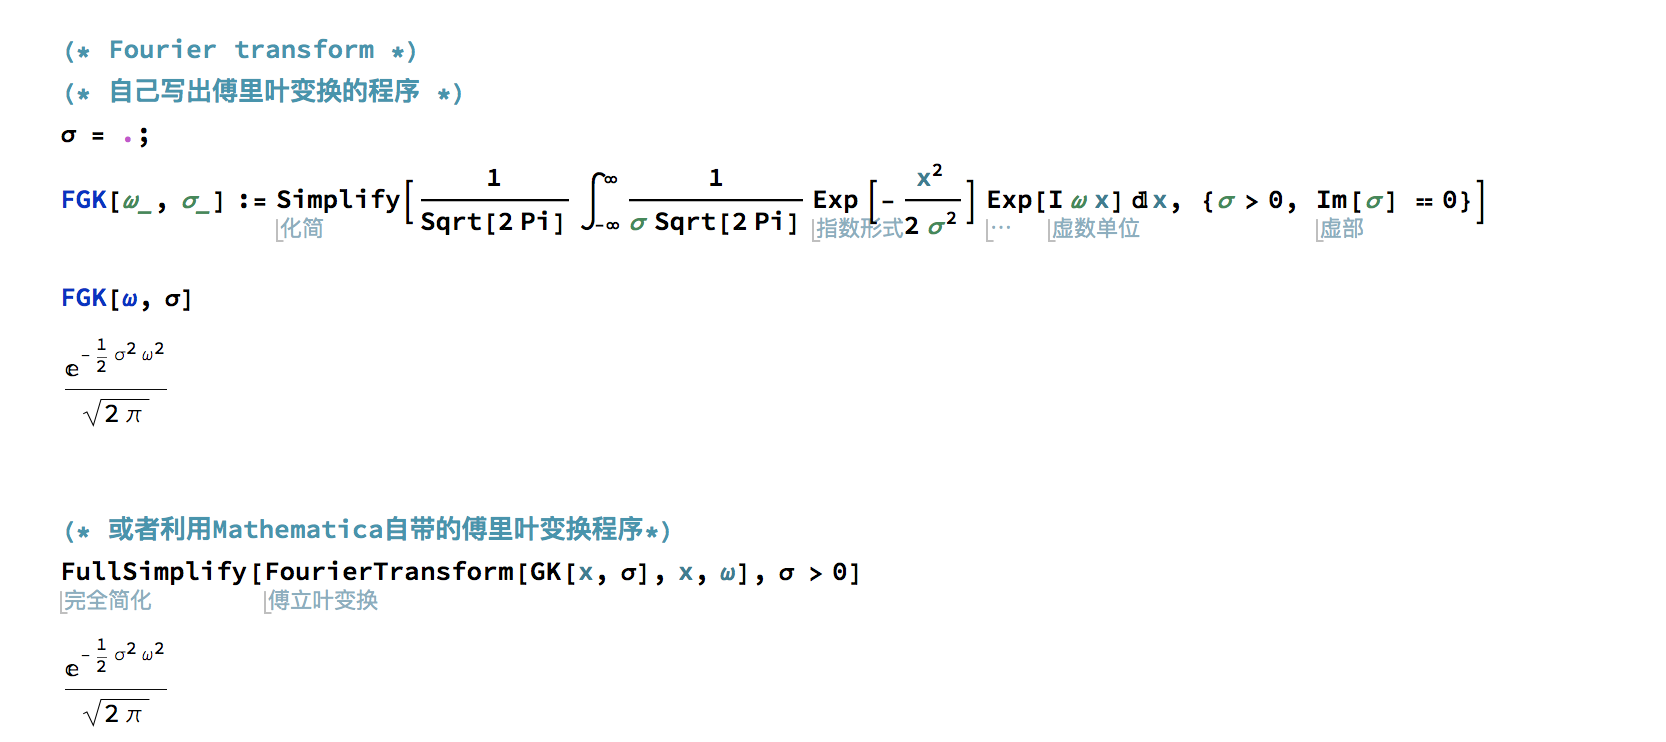
\includegraphics[width=12cm]{./Figures/20180405-fourier-transform-mma}
  \label{fig:fourier-transform-mma.png}
%
%  \small{Source: PBOC.}
\end{figure}

不难看出,对高斯核方程的傅里叶变换还是一个傅里叶变换,只是频率变化为$\omega$。这一特性为高斯核方程所独有。原域中的带宽(方差)系数$\sigma$,在新的傅里叶变换中表现为和频率$\omega$相乘的形式出现。$\sigma$值越大,方差越大,高斯核越宽,其对应的傅里叶域中的核越窄,$\omega$越小,如下图\ref{fig:fourier-transform-kernel-compare.png},从左至右分别对应$\sigma = 1,2,3$,从上到下分别是原域中的高斯核方程,以及对应的傅里叶变换。

\begin{figure}[htbp]
  \caption{傅里叶变换、逆傅里叶变换的Mathematica程序}
  \centering
  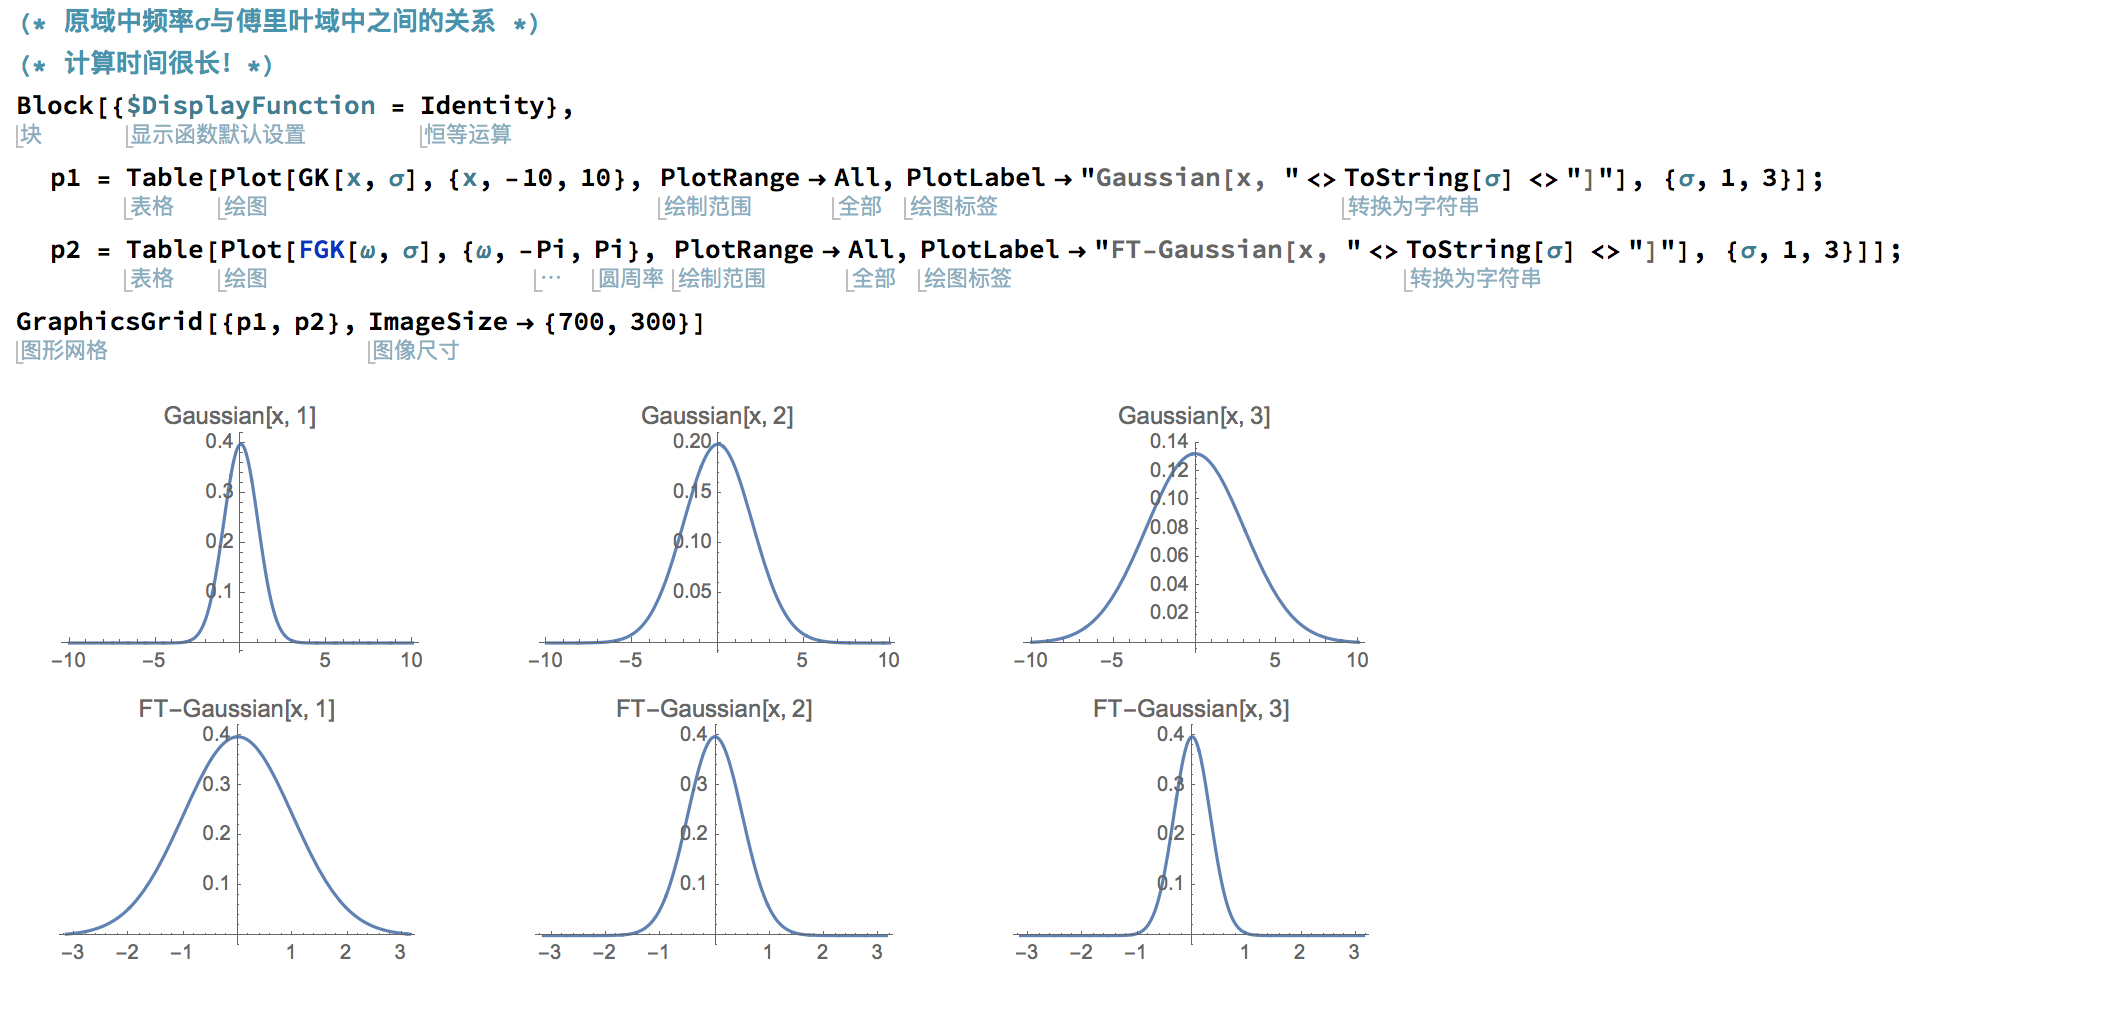
\includegraphics[width=15cm]{./Figures/20180405-kernel-compare.png}
  \label{fig:fourier-transform-kernel-compare.png}
%
%  \small{Source: PBOC.}
\end{figure}

对高斯核方程$G(x;\sigma)$的傅里叶变换$\mathcal{F} g(x;\sigma)$,有许多种不同的称谓,若$g(x;\sigma)$是信号,那么$\mathcal{F} g(x;\sigma)$可称为光谱(spectrum),起到滤波的作用,又称带宽滤波(bandpass filter, BPF)\index{bandpass filter (BPF) \dotfill 带宽滤波}。


%!TEX root = ../DSGEnotes.tex

\section{数值线性代数基础}
\label{sec:numlin}

\subsection{矩阵结构与算法复杂度}
\label{sec:numlin-matrix-structure-algorithm-complexity}

以如下线性方程的求解为例
\begin{equation}
  \label{eq:numlin-matrix-example}
  \underbrace{A}_{\left(n \times n \right)}
  \underbrace{x}_{\left( n \times 1 \right)}
  = \underbrace{b}_{\left( 1 \times 1 \right)},
\end{equation}
假设$A$是非奇异矩阵(nonsingular matrix, Proposition \ref{prop:simple-schur-quadratic-optim}),以确保对于所有$b$的值,方程都有唯一解$x = A^{-1} b$。$A$表示系数矩阵。RHS的$b$设为一个常数(随后我们会讨论更复杂一些的情况,比如$b$是一个向量)。

数值近似所需的时间通常以$n^{3}$计。本节介绍的线性方程系统的通用求解方法,在对实时性要求不高,或者$n$值不太大(如$<10^{3}$)的情况下,通常是有效的。

系数矩阵的结构问题。在通常情况下,我们可以设系数矩阵$A$具有一些特殊形式,以提高数值求解的效率(速度),尤其是在$n$值较大时,效率的提升可能会很明显。$A$可供选择的形式有很多种,较简单的包括密集矩阵,和稀疏形式的矩阵等\footnote{较为复杂的矩阵形式暂不讨论,如Toeplitz, Hankel, Circulant matrix等。},稀疏形如
\begin{itemize}
  \item 带状矩阵(band matrix),
  \item 块对角矩阵(block diagonal matrix),
  \item 稀疏矩阵(sparse matrix),由$0$和非零元素共同构成的矩阵等。
\end{itemize}

下面以密集形矩阵为例,介绍通用解法。在介绍之前,先来看一下算法复杂度(求解效率)的判定标准。

\subsection*{利用flops指标作复杂度分析}
数值近似计算过程中常用浮点计算数flop(floating points operations, flops)\index{flops!(floating points operations) \dotfill 浮点计算数}作为测度计算效率的指标。例如求解
\begin{equation*}
  m^{3} + 3 m^{3} n + mn + 4 m n^{2} + 5m + 22
\end{equation*}
所需的浮点计算数量。需要指出的是,在统计flops时常常只统计幂次较高的项,即含有最高幂次或者主要部分的项,的浮点运算次数,而忽略余下的部分。在上例的数值求解过程中,统计flops只需要考虑$m^{3} + 3 m^{2} n + 4 m n^{2}$的部分即可;如果$m << n$,那么只需计算$4 m n^{2}$部分即可。

现在来看基础矩阵——向量运算的成本。以计算内积$\langle x, y \rangle$为例,向量$x,y \in \mathbb{R}^{n}$:第一步需要执行$x_{i} \times y_{i} \forall i \in n$,共需$(n)$ flops。然后将各项加总,需 $(n-1)$ flops,一共 $(2n-1)$ flops。若只统计首项,$2n$ flops。或者更简单些,只考虑幂次,$n$ flops。

\subsubsection*{标量——矩阵乘积形式}
$\alpha x, \, \alpha \in \mathbb{R}, \, x \in \mathbb{R}^{n}$,$n$ flops。

$x + y$, $n$ flops。

如果$x$和$y$是稀疏矩阵,即均含有一些非零元素,那么计算速度可能更快。例如若$x$中的非零元素数量是$N$,则$\langle x,y \rangle = x^{\top} y $,有$2N$ flops。

\subsubsection*{矩阵——向量乘积形式}
以计算下式为例
\begin{equation*}
  \underbrace{y}_{\left( m \times 1 \right)}
  = \underbrace{A}_{\left( m \times n \right)}
  \underbrace{x}_{\left( n \times 1 \right)},
\end{equation*}
$2 mn$ flops。

$A$的特殊形式可以提升计算速度,如
\begin{itemize}
  \item $A$是对角矩阵,那么 $A x$计算需 $n$ flops,
  \item $A$是系数矩阵,其中包括$N$个非零元素,那么 $A x$计算需 $2N$ flops。
\end{itemize}

如果设$A$的秩满足$\rank (A) \le \min \left\{ m, n \right\}$,并且$A$可以分解为
\begin{equation*}
  \underbrace{A}_{\left( m \times n \right)}
  = \underbrace{U}_{\left( m \times p \right)}
  \underbrace{V}_{\left( p \times n \right)},
\end{equation*}
那么可以首先计算 $V x$ ($2pn$ flops),再计算$U \left( Vx \right)$ ($2mp$ flops),总共$2 \left( m+n \right) p << 2 mn$ flops。

\subsubsection*{矩阵——矩阵乘积形式}
来看
\begin{equation*}
  \underbrace{C}_{\left( m \times p \right)} =
  \underbrace{A}_{\left( m \times n \right)}
  \underbrace{B}_{\left( n \times p \right)},
\end{equation*}
$2 m n p$ flops。

\subsection{矩阵结构与线性系统求解}
\label{sec:numlin-decomposition}

先从较简单的线性系统\eqref{eq:numlin-matrix-example}求解开始。

\subsubsection{对角矩阵}
\label{sec:numlin-matrix-diagonal}
设$A$是对角矩阵(diagonal matrix)\index{matrix!diagonal \dotfill 对角矩阵},非奇异,即矩阵中元素满足$a_{ii} \neq 0 \, \forall i \in n$。那么有
\begin{equation*}
  a x = b \Leftrightarrow a_{ii} x_{i} = b_{i}, \, i = 1,\ldots,n,
\end{equation*}
对应的解$\left\{ x_{i} \right\}_{i \in n}$满足
\begin{equation*}
  x_{i} = \frac{b_{i}}{a_{ii}}, \quad i=1,\ldots,n,
\end{equation*}
$n$ flops.

\subsubsection{下三角矩阵}
若$A \in \mathbb{R}^{n \times n}$满足$a_{i,j} \, \forall j > i, \, i,j=1,\ldots,n$,我们称之为下三角矩阵(lower triangular matrix)\index{matrix!triangular, lower \dotfill 下三角矩阵}。若下三角矩阵中的所有非零元素的值都为$1$,则称为单位下三角矩阵(unit lower triangular matrix)\index{matrix!triangular, unit lower \dotfill 下三角单位矩阵},例如一个$5 \times 5$的单位下三角矩阵
\begin{equation*}
\begin{pmatrix}
   1 & 0 & 0 & 0 & 0\\
   1 & 1 & 0 & 0 & 0\\
   1 & 1 & 1 & 0 & 0\\
   1 & 1 & 1 & 1 & 0\\
   1 & 1 & 1 & 1 & 1
 \end{pmatrix}.
\end{equation*}

当且仅当下三角矩阵$A$的全部对角元素不为$0$,即$a_{ii} \neq 0 \, \forall i =1,\ldots,n$时,$A$才是一个非奇异矩阵。

非奇异下三角矩阵$A$代回原式,有
\begin{equation*}
  \begin{pmatrix}
  a_{11} & 0 & \ldots & 0 \\
  a_{21} & a_{22} &\ldots & 0 \\
  \vdots & \ddots & \ddots & 0\\
  a_{n1} & a_{n2} & \ldots & a_{nn}
\end{pmatrix}
\,
\begin{pmatrix}
  x_{1} \\ x_{2} \\ \vdots \\ x_{n}
\end{pmatrix}
=
\begin{pmatrix}
  b_{1} \\
  b_{2} \\
  \vdots \\
  b_{n}
\end{pmatrix}.
\end{equation*}

求解,依次有
\begin{equation*}
  \begin{split}
    x_{1} & = \frac{b_{1}}{a_{11}}, \quad (1 flops)\\
    x_{2} & = \frac{b_{2} - a_{21} x_{1}}{a_{22}}, \quad (3 flops)\\
    x_{3} & = \frac{b_{3} - a_{31} x_{1} - a_{32} x_{2}}{a_{33}}, \quad (5 flops)\\
    \vdots & \\
    x_{n} & = \frac{
    b_{n} - a_{n1} x_{1} - a_{n2} x_{2} - \ldots - a_{n,n-1} x_{n-1}
    }{
    a_{nn}
    }, \quad (2n-1 flops)
  \end{split}
\end{equation*}
这种求解思路称向前替换(forward subsititution),即在每一个计算$x_{i}$的过程中,将已求解得到的$x_{1},x_{2},\ldots,x_{i-1}$作为已知量代入。总共需要计算
\begin{equation*}
  \Sigma = 1 + 3 + 5 + \ldots + \left( 2 n - 1 \right)
  = n^{2} flops.
\end{equation*}

如果$A$除了下三角、非奇异之外还有其他更多一些特征,我们可以进一步优化算法,提高求解效率,使得计算数低于$n^{2}$。例如若$A$还是稀疏的或带状的,每一行中有不超过$k$个元素,则向前替代需要$\left( 2k+1 \right)$flops,总计$\left( 2k + 1 \right) n$ flops,以首项记为$\left( 2kn \right)$次。


\subsubsection{上三角矩阵}
若$A \in \mathbb{R}^{n \times n}$的转置$A^{\top}$是个下三角矩阵,满足$a_{i,j} =0 \, \forall i > j, \, i,j=1,\ldots,n$,我们称之为上三角矩阵(upper triangular matrix)\index{matrix!triangular, upper \dotfill 上三角矩阵}。若上三角矩阵中的所有非零元素的值都为$1$,则称为单位上三角矩阵(unit upper triangular matrix)\index{matrix!triangular, unit upper \dotfill 上三角单位矩阵}。

对应的求解过程为向后替代(backward substitution)
\begin{equation*}
\begin{split}
    x_{n} & = \frac{b_{n}}{a_{n-1}}, \\
    x_{n-1} & = \frac{
    b_{n-1} - a_{n-1,n} x_{n} x_{n}
    }{
    a_{n-1,n-1}
    }, \\
    x_{n-2} & = \frac{
    b_{n-2} - a_{n-2,n-1} x_{n-1} - a_{n-2,n} x_{n}
    }{
    a_{n-2,n-2}
    }, \\
    \vdots & \\
    x_{1} & = \frac{
    b_{1} - a_{12}x_{2} - a_{13}x_{3} - \ldots - a_{1n}x_{n}
    }{
    a_{11}
    },
\end{split}
\end{equation*}
也是$n^{2}$ flops。若$A$稀疏,每一行最多有$k$个非零元素,那么 $\left(2 kn \right)$ flops。

\subsubsection{正交矩阵}
\label{sec:numlin-matrix-orthogonality}
$A \in \mathbb{R}^{n \times n}$若满足如下条件,我们称之为正交矩阵(orthogonal matrix)\index{matrix!orthogonal \dotfill 正交矩阵}
\begin{equation*}
  A^{\top} \, A = I, \quad \text{即 } \, A^{-1} = A^{\top}.
\end{equation*}

此时线性系统$A x = b$为
\begin{equation*}
  x = A^{-1} b = A^{\top} b, \quad \left( 2n^{2} \right) \, flops.
\end{equation*}

若正交矩阵还具有更多属性如
\begin{equation*}
  A = I - 2 \, u \, u^{\top}, \quad \left\| u \right\|_{2} = 1,
\end{equation*}
那么
\begin{equation*}
  \begin{split}
    x & = A^{-1} b = \left( I - 2 \, u \, u^{\top} \right)^{\top} \,
    = b - 2 \, u^{\top} \, b \, u,
    \end{split}
\end{equation*}
计算步骤
\begin{itemize}
  \item 算$u^{\top} \, b$,$\left( n \right)$ flops,
  \item 算$u^{\top} \, b \, u $,$\left( n \right)$ flops,
  \item 算$-2 \, u^{\top} \, b \, u $,$\left( n \right)$ flops,
  \item 算$b - 2 \, u^{\top} \, b \, u$, $\left( n \right)$ flops,
\end{itemize}
$\Sigma = 4n$ flops。

\subsubsection{置换矩阵}
\label{sec:numlin-matrix-permutation}
置换矩阵(permutation matrix)\index{matrix!permutation \dotfill 置换矩阵}是指只由$0$和$1$组成的方块矩阵,每一行和每一列都有且只有一个$1$,其余均为$0$。在线性代数中,每个$n$元置换矩阵都代表一个对$n$个元素的置换,这$n$个元素常常是$n$维空间的基。当一个矩阵乘以一个置换矩阵时,得到的是原矩阵的行(若置换矩阵在左)或列(若置换矩阵在右)经过置换后的矩阵。具体说来,每个$n$元置换都对应唯一的一个置换矩阵。设$\pi$为一个$n$元置换$\pi: \left\{ 1,\ldots,n \right\} \mapsto \left\{ 1, n \right\}$,对应映射图
\begin{equation*}
  \begin{pmatrix}
    1 & 2 & \ldots & n \\
    \pi(1) & \pi(2) & \ldots & \pi(n)
  \end{pmatrix},
\end{equation*}
那么它的$n \times n$置换矩阵$P_{\pi}$是指,在第$i$行上只有$\pi(i)$位置上的系数是$1$,其余均为$0$:
\begin{equation}
  \label{eq:numlin-matrix-permutation}
  P_{\pi} = \begin{pmatrix}
  e_{\pi(1)} \\e_{\pi(2)} \\ \vdots \\ e_{\pi(n)}
  \end{pmatrix},
\end{equation}
其中$e_{j}$表示正则基中的第$j$个,也即第$j$行左起第$j$个元素是$1$,其余均为$0$。

此外设一个单位矩阵(identity matrix)\index{matrix!identity \dotfill 单位矩阵} $I \in \mathbb{R}^{n \times n} = \left[ e_{1}, e_{2}, e_{3}, \ldots, e_{n} \right]^{\top}$,因此置换矩阵也可以看做是对单位矩阵的某些行和列交换后所得到的矩阵。

置换矩阵具有一些性质如下
\begin{enumerate}
  \item 设2个$n$元置换$\pi$和$\sigma$,分别对应2个$n \times n$置换矩阵$P_{\pi}, \, P_{\sigma}$,那么
  \begin{equation*}
    P_{\pi} P_{\sigma} = P_{\pi \, \sigma}.
  \end{equation*}
  \item 一个置换矩阵必然是正交矩阵,满足
  \begin{equation*}
    P_{\pi} \, P_{\pi}^{\top} = I,
  \end{equation*}
  并且它的逆矩阵也是一个置换矩阵
  \begin{equation*}
    P_{\pi}^{-1} = P_{\pi^{-1}} = P_{\pi}^{\top}.
  \end{equation*}
\end{enumerate}

左乘:置换矩阵$P_{\pi}$左乘一个列向量$g$,得到的是$g$的系数经置换后的新向量
\begin{equation*}
  P_{\pi} \, g=
  \begin{pmatrix}
    e_{\pi(1)} \\
    e_{\pi(2)} \\
    \vdots \\
    e_{\pi(n)} \\
  \end{pmatrix}
  \,
  \begin{pmatrix}
    g_{1} \\ g_{2} \\ \vdots \\ g_{n}
  \end{pmatrix}
  =
  \begin{pmatrix}
    g_{\pi^(1)} \\
    g_{\pi(2)} \\
    \vdots \\
    g_{\pi(n)} \\
  \end{pmatrix}.
\end{equation*}

右乘:置换矩阵$P_{\pi}$右乘一个行向量$h$,得到的是$h$的系数经置换后的新向量
\begin{equation*}
  h \,   P_{\pi} =
  \begin{pmatrix}
    h_{1} , h_{2} , \ldots , h_{n}
  \end{pmatrix}
  \,
  \begin{pmatrix}
    e_{\pi(1)} \\
    e_{\pi(2)} \\
    \vdots \\
    e_{\pi(n)} \\
  \end{pmatrix}
  =
  \begin{pmatrix}
    h_{\pi^{-1}(1)} ,
    h_{\pi^{-1}(2)} ,
    \ldots,
    h_{\pi^{-1}(n)}
  \end{pmatrix}.
\end{equation*}

例如$\pi= (1,4,2,5,3)$,对应映射
\begin{equation*}
  \begin{pmatrix}
    1 & 2 & 3 & 4 & 5 \\
    1 & 4 & 2 & 5 & 3
  \end{pmatrix},
\end{equation*}
建立置换矩阵
\begin{equation*}
  P_{\pi} =
  \begin{pmatrix}
    e_{\pi(1)} \\
    e_{\pi(2)} \\
    e_{\pi(3)} \\
    e_{\pi(4)} \\
    e_{\pi(5)}
  \end{pmatrix}
  = \begin{pmatrix}
  e_{1} \\ e_{2} \\ e_{3} \\ e_{4} \\ e_{5}
  \end{pmatrix}
  = \begin{pmatrix}
  1 & 0 & 0 & 0 & 0 \\
  0 & 0 & 0 & 1 & 0 \\
  0 & 1 & 0 & 0 & 0 \\
  0 & 0 & 0 & 0 & 1 \\
  0 & 0 & 1 & 0 & 0
  \end{pmatrix}.
\end{equation*}

对于一个给定的向量$g = \left[ g_{1}, g_{2}, g_{3}, g_{4}, g_{5} \right]^{\top}$,我们有
\begin{equation*}
  P_{\pi} \, g =
  \begin{pmatrix}
    e_{\pi(1)} \\
    e_{\pi(2)} \\
    e_{\pi(3)} \\
    e_{\pi(4)} \\
    e_{\pi(5)}
  \end{pmatrix}
  \,
  \begin{pmatrix}
    g_{1} \\
    g_{2} \\
    g_{3} \\
    g_{4} \\
    g_{5}
    \end{pmatrix}
    =
    \begin{pmatrix}
    e_{1} \\ e_{2} \\ e_{3} \\ e_{4} \\ e_{5}
    \end{pmatrix}
    \,
    \begin{pmatrix}
      g_{1} \\
      g_{2} \\
      g_{3} \\
      g_{4} \\
      g_{5}
      \end{pmatrix}
    = \begin{pmatrix}
    g_{1} \\ g_{4} \\ g_{2} \\ g_{5} \\ g_{3}
    \end{pmatrix}.
\end{equation*}

回到本节$Ax=b$的求解问题。如果$A$是一个转置矩阵,那么求解方法为,对向量$b$做$\pi^{-1}$的置换:
\begin{equation*}
  x = A_{\pi^{-1}} b = A^{T} b, \quad \left( 0 \right) flops.
\end{equation*}
虽然仍然涉及到浮点数的复制粘贴,但计为$0$。

\subsection{矩阵分解}
\label{sec:numlin-matrix-factorization}
在实际求解线性系统的过程中,有时很难第一眼就看出系数矩阵$A$具有哪些特殊结构。这时可以尝试将它分解为一组非奇异矩阵的乘
\begin{equation}
  \label{eq:numlin-matrix-factorization-fact-step}
\begin{split}
    & A = A_{1} \, A_{2} \, \ldots A_{k}, \\
    \hookrightarrow & A x = b \Leftrightarrow x = A^{-1} b
    = A_{k}^{-1} \, A_{k-1}^{-1} \, \ldots A_{1}^{-1} \, b.
\end{split}
\end{equation}

可以从右向左求解
\begin{equation}
\label{eq:numlin-matrix-factorization-solution-step}
\begin{split}
    z_{1} & = A_{1}^{-1} b, \\
    z_{2} & = A_{2}^{-1} z_{1} = A_{2}^{-1} A_{1}^{-1} b, \\
    \vdots & \\
    z_{i} &= A_{i}^{-1} z_{i-1} = A_{i}^{-1} A_{i-1}^{-1} \ldots A_{1}^{-1} b,
\end{split}
\end{equation}

在此基础上进一步计算系统的解$x$
\begin{equation*}
  x = A_{k}^{-1} z_{k-1} = A_{k}^{-1} A_{k-1}^{-1} \ldots A_{1}^{-1} b.
\end{equation*}

这种方法称为矩阵的因子分解(factorization)。如果$A_{i}$具有较好的结构,比如是(上或下)对角矩阵、置换矩阵等,那么分解法可用于高效求解线性系统$A x = b$。有时为了记忆方便,对于将系数矩阵做分解$A=A_{1} \ldots A_{i}$的计算过程\eqref{eq:numlin-matrix-factorization-fact-step}称为分解步骤(factorization step),对应 $f$ flops。对于求解$z_{i} = A_{i}^{-1} z_{i-1}$ \eqref{eq:numlin-matrix-factorization-solution-step}的步骤称为求解步骤(solution step),对应 $s$ flops。通常来说,求解步骤所需成本远高于分解步骤,$f >> s$。

现在作个扩展,$b$不再是个常数而是个向量,对应线性系统
\begin{equation*}
\begin{split}
  & A X = B,  \\
  & A \in \mathbb{R}^{n \times n}, \\
  & X = \left[ x_{1}, x_{2}, \ldots, x_{m} \right] \in \mathbb{R}^{ n \times m}, \\
  & B = \left[ b_{1}, b_{2}, \ldots, b_{m} \right] \in \mathbb{R}^{ n \times m}.
\end{split}
\end{equation*}

求解方法类似:$A$的分解步骤需要 $f$ flops;随后对$1,\ldots,m$分别求解$A_{i}^{-1} b_{i}$,一共需要 $(m s)$ flops,$\Sigma = \left( f + ms \right)$ flps,并且往往$f >> s$。

下面介绍一些常见的因子分解法,如LU分解,Cholesky分解,$LDL^{\top}$分解等。

\subsection{LU因子分解}
\label{sec:numlin-factorization-lu}
任意一个非奇异矩阵$A \in \mathbb{R}^{n \times n}$都可以分解为PLU的形式
\begin{equation}
  A = P \, L \, U,
\end{equation}
其中$P \in \mathbb{R}^{n \times n}$是置换矩阵,$L, U \in \mathbb{R}^{n \times n}$分别是上、下三角矩阵,这种方法称为$A$的LU分解(LU factorization)\index{matrix factorization!LU \dotfill LU分解}。结合转置矩阵的特征,上式可改写为
\begin{equation}
  \label{eq:numlin-factorization-lu}
  P^{\top} A = LU,
\end{equation}
数值计算求解LU分解的标准算法是高斯部分主元消除法(Gaussian elimination of partial pivoting),又称高斯行主元消除法(Gaussian elimination of row pivoting)\index{Gaussian elimination \dotfill 高斯消元},消耗 $\frac{2}{3} n^{3}$ flops。

\subsubsection{利用LU分解法求解线性方程系统}
LU分解+分解步和求解步,是线性方程系统如$Ax=b$的标准求解方法。
\begin{algorithm}[利用LU分解法求解线性方程系统]
  \label{algorithm:numlin-factorization-lu}
  给定一个线性方程系统$Ax=b$,其中系数矩阵$A$非奇异,$b$是个常数,经典的求解步骤如下:
  \begin{enumerate}
    \item LU因式分解,将$A$分解为$A = P \, L \, U$,$\left( \frac{2}{3} n^{3} \right)$ flops。
    \item 置换,求解$P z_{1} = b$, $(0)$ flops。
    \item 向前替换,求解$L \, z_{2} = z_{1}$, $\left( n^{2} \right)$ flops。
    \item 向后替换,求解$U \, x = z_{2}$, $ \left( n^{2} \right)$ flops。
  \end{enumerate}

  总共消耗$\left( \frac{2}{3} n^{3} + 3 n^{2} \right)$ flops。
\end{algorithm}

如果$b \in \mathbb{R}^{n}$是一个向量,整个系统变成一个由$m$个方程组成的线性系统$A x_{i} = b_{i}, \, i = 1,\ldots,m$,计算方法类似,消耗成本$\left( \frac{2}{3} n^{3} + 2 m n^{2} \right)$ flops。

如果非奇异矩阵$A$还具有其他一些额外的性质,如带状或系数,则可通过优化算法提高数值计算的效率。

若$A$是带状矩阵(band matrix)\index{matrix!band \dotfill 带状矩阵},指
\begin{equation}
  \label{eq:numlin-band-matrix-def}
  a_{ij} = 0, \quad \text{如果 } \left| i - j \right| > k,
\end{equation}
其中$k < n-1$,称为$A$的带宽(bandwidth)\index{bandwidth (matrix) \dotfill 带宽(矩阵的)}。对于$k << n$的情况,计算消耗$\left( 4 n k^{2} \right)$ flops。

若$A$是稀疏矩阵,那么其LU因子分解中常常同时既含有行置换,也含有列置换,即
\begin{equation*}
  A = P_{1} \, L \, U \, P_{2},
\end{equation*}
其中$P_{1}, \, P_{2}$都是置换矩阵。这时采用LU因子分解会大大提升计算效率,L和U的稀疏程度取决于$P_{1}$和$P_{2}$的具体形式。

\subsection{Cholesky因子分解}
\label{sec:numlin-factorization-cholesky}
如果$A \in \mathbb{R}^{n \times n}$是对称且正半定的矩阵,那么可以因子分解为
\begin{equation}
  \label{eq:numlin-factorization-cholesky}
  A = L \, L^{\top},
\end{equation}
其中L是下三角矩阵,非奇异,且对角元素值为正。这称为$A$的Cholesky因子分解(Cholesky factorization)\index{matrix factorization!Cholesky \dotfill Cholesky分解}。当不对$A$作任何结构优化时,消耗$ \left( \frac{1}{3} n^{3} \right)$ flops。

\begin{algorithm}[利用Cholesky分解求解正定线性方程系统]
  \label{algorithm:numlin-factorization-cholesky}
给定一组线性方程系统$A x = b$,其中系数矩阵$A$对称,正半定。那么利用Cholesky分解求解系统的算法如下
\begin{enumerate}
  \item Cholesky因子分解,$A = L \, L^{\top}$,$\left( \frac{1}{3} n^{3} \right)$ flops。
  \item 向前替代,求解$L \, z_{1} = b$,$\left( n^{2} \right)$ flops。
  \item 向后替代,求解$L^{\top} x = z_{1}$,$\left( n^{2} \right)$ flops。
\end{enumerate}
$\Sigma = \frac{1}{3} n^{3} + 2 n^{2} \approx \frac{1}{3} n^{3}$ flops。
\end{algorithm}

若$A$还具有进一步的特殊结构,则计算效率可进一步提高。如果$A$对称、正半定且是个带宽为$k$的带状矩阵,计算消耗$\left(n k^{2} \right)$ flops。

如果$A$对称、正半定且是个稀疏矩阵$A = P \, L \, L^{\top} \, P^{\top}$,那么等价于
\begin{equation*}
  P^{\top} \, A \, P = L \, L^{\top},
\end{equation*}
换句话说,$\left( P^{\top} A P \right)$的Cholesky因子分解是$L \, L^{\top}$。

原则上来说,我们可以选择任意形式的置换矩阵$P$,每1个$P$都有唯一的$L$相对应,但不同$P$的选择会大大影响数值求解的效率。对此,常常需要采用不同的启发式方法来选取最合适、或者更合适的置换矩阵类型。例如当$A$是一个稀疏型矩阵
\begin{equation*}
  A = \begin{pmatrix}
  1 & u^{\top} \\ u & D
  \end{pmatrix},
\end{equation*}
其中$D \in \mathbb{R}^{n \times n}$是正对角矩阵,$u \in \mathbb{R}^{n}$。

$A$正定要求满足$\det A >0$
\begin{equation*}
  \begin{split}
    & \det A = D - u \, u^{\top} > 0, \\
    \hookrightarrow & D > u \, u^{\top}, \\
    \hookrightarrow & u^{\top} D^{-1} u < 1,
  \end{split}
\end{equation*}

对$A$的Cholesky因子分解可写作
\begin{equation}
  \label{eq:umlin-factorization-cholesky-a}
  \begin{pmatrix}
    1 & u^{\top} \\ u &  D
  \end{pmatrix}
  = \begin{pmatrix}
  1 & 0 \\ u & L
  \end{pmatrix}
  \, \begin{pmatrix}
  1 & u^{\top} \\ 0 & L^{\top}
  \end{pmatrix},
\end{equation}
其中$L$是下三角矩阵,满足
\begin{equation*}
  L \, L^{\top} = D - u \, u^{\top}.
\end{equation*}

对于一般形式的$u$而言,矩阵$\left( D - u \, u^{\top} \right)$是密集矩阵,因此可以判定$L$也是密集矩阵。那么,尽管$A$可能是非常稀疏的(比如大多数行只有两个非零元素),其Cholesky因子$L$却仍是密集的。

另一方面,假设我们将$A$的第1行、第1列置换到最后1行、最后1列,重新排序后做Cholesky因子分解,可得
\begin{equation}
  \label{eq:umlin-factorization-cholesky-a-redo}
\begin{pmatrix}
  D & u \\
  u^{\top} & 1
\end{pmatrix}
= \begin{pmatrix}
D^{\frac{1}{2}} & 0 \\
u^{\top} \, D^{-\frac{1}{2}} & \left( 1 - u^{\top} \, D^{-1} \, u \right)^{\frac{1}{2}}
\end{pmatrix}
\,
\begin{pmatrix}
  D^{\frac{1}{2}} & D^{-\frac{1}{2}} \, u \\
  0 & \left( 1 - u^{\top} \, D^{-1} \, u \right)^{\frac{1}{2}}
\end{pmatrix}
\end{equation}

由\eqref{eq:umlin-factorization-cholesky-a} \eqref{eq:umlin-factorization-cholesky-a-redo}可见,Cholesky因子$L$的对角块是$(1,1)$,因此也是密集的。

这个例子表明,重新排序可以极大改变Cholesky因子的稀疏性。很显然,``最好"的置换方案,或者退一步说,所有``理想"的排序方法,都是将密集的行和列置换到末尾。所谓``理想"的方法,是指较为复杂的稀疏型矩阵也许很难找到最优的置换方案,即,使得$L$中的$0$元素个数达到最大,但还是有一些启发式方案可以追求次优。

在系数矩阵作Cholesky因子分解过程中,$P$的选取往往只根据$A$的稀疏结构进行,而不取决于$A$中非零元素的具体数值%\todo{与下文 $LDL^{\top}$分解法做比较}
\footnote{与之相比较,对稀疏矩阵作$LU$分解的过程中,$P$的选取则不只取决于$A$的稀疏结构,还取决于$A$中非零元素的具体值。}。而一旦确定了$P$,我们就可以算得唯一的$L$的系数结构,也不取决于$A$中非零元素的具体数值。这成为$A$的符号因子分解(symbolic factorization step),作为求解稀疏矩阵系统的第一个步骤。第二步是数值因子分解,即计算$L$中非零元素的值。常见的计算Cholesky因子分解的软件常常将这两个步骤的计算过程分别处理,这在大多数情况下是有必要的:第一步的计算成本往往高于第二步。

\subsection[LDL因子分解]{$LDL^{\top}$因子分解}
\label{sec:numlin-factorization-ldl}
每个非奇异对称矩阵$A$都可因式分解为如下形式
\begin{equation}
  \label{eq:numlin-factorization-ldl}
  A = P \, L \, D \, L^{\top} \, P^{\top},
\end{equation}
其中$P$是置换矩阵,$L$是对角元素均为正的下三角矩阵,$D$是块对角矩阵,对角块由$1 \times 1$和$2 \times 2$的非奇异对角块构成。这称为$A$的$LDL^{\top}$因子分解(LDL factorization)\index{matrix factorization!$LDL^{\top}$ \dotfill $LDL^{\top}$分解}。

Cholesky分解可以被视为是一种特殊形式的$LDL^{\top}$分解:$P=I, \, D = I$。

\begin{algorithm}[利用$LDL^{\top}$分解求解线性方程系统]
  \label{algorithm:numlin-factorization-ldl}
  给定一个线性方程$A x = b$,其中$A$非奇异。$LDL^{\top}$法求解步骤如下
  \begin{enumerate}
    \item $LDL^{\top}$因子分解,$A = P \, L \, D \, L^{\top} \, P^{\top}$, $\left( \frac{1}{3} n^{3} \right)$ flops。
    \item 置换,求解$P \, z_{1} = b$, $\left( 0 \right)$ flops。
    \item 向前替换,求解$L z_{2} = z_{1}$, $\left( n^{2} \right)$ flops。
    \item 对角块元素求解,求解$D \, z_{3} = z_{2}$, $\left( n \right)$ flps。
    \item 向后替换,求解$L^{\top} z_{4} = z_{3}$, $\left( n^{2} \right)$ flops。
    \item 置换,求解$P^{\top} x = z_{4}$, $\left( 0 \right)$ flps。
  \end{enumerate}
\end{algorithm}

当$A$具有一些特殊结构,如带状矩阵或系数矩阵时,可以进一步提高计算效率。调整过程与Cholesky因子分解的过程相似,只是要额外多考虑一个对角块$D$。此外,$LDL^{\top}$因子分解过程中,在选取$P$时,除了要(像稀疏Choleky分解那样)考虑稀疏矩阵的结构特征之外,还要考虑矩阵$A$中非零元素的值。

\subsection{块消除与Schur补}
\label{sec:numlin-block-elimination}

\subsubsection{变量块的高斯消元}
\label{sec:numlin-gaussian-elimination}
求解线性方程系统$A x = b$的过程中,一种常用的方法是,首先利用一定方法小区部分变量元素,将剩下的变量元素组成一个更小的线性方程系统,以便提高数值计算的效率。

若$A$是一个没有明显规律的密集矩阵,这种方法很难带来计算效率的提升。然而若$A$中的某一部分子矩阵含有可消除变量,易于作因子分解(例如是快对角或带状结构的),那么应用这种方法会带来效率的显著提升。

假定我们将$x \in \mathbb{R}^{n}$分为以下2个块(子向量)
\begin{equation*}
  \underbrace{x}_{\left( \left( n_{1} + n_{2} \right) \times 1 \right)} =
  \begin{pmatrix}
  \underbrace{x_{1}}_{\left( n_{1} \times 1 \right)} \\
  \underbrace{x_{2}}_{\left( n_{2} \times 1 \right)}
  \end{pmatrix},
\end{equation*}

相应地,待求解线性系统变为
\begin{equation}
  \label{eq:numlin-gaussian-elimination}
  A x = b \Longleftrightarrow
  \begin{pmatrix}
    \underbrace{A_{11}}_{\left( n_{1} \times n_{1} \right)} &
    \underbrace{A_{12}}_{\left( n_{1} \times n_{2} \right)} \\
    \underbrace{A_{21}}_{\left( n_{2} \times n_{1} \right)}&
    \underbrace{A_{22}}_{\left( n_{2} \times n_{2} \right)}
  \end{pmatrix}
  \,
  \begin{pmatrix}
    x_{1} \\ x_{2}
  \end{pmatrix}
  =
  \begin{pmatrix}
      b_{1} \\
      b_{2}
  \end{pmatrix}.
\end{equation}

若假定子矩阵$A_{11}$可逆,则可以采用如下方法,从线性方程中消去$A_{11}$:由第一行方程有
\begin{equation}
  \label{eq:numlin-gaussian-elimination-row1}
  \begin{split}
    & A_{11} x_{1} + A_{12} x_{2} = b_{1}, \\
    \hookrightarrow & x_{1} = \frac{b_{1} - A_{12} x_{2}}{A_{11}}.
  \end{split}
\end{equation}

代入第二行方程替换掉其中的$x_{1}$
\begin{equation}
  \label{eq:numlin-gaussian-elimination-row2}
  \begin{split}
    & A_{21} x_{1} + A_{22} x_{2} = b_{2}, \\
    \hookrightarrow &
    \underbrace{
    \left( A_{22} - A_{21} A_{11}^{-1} A_{12} \right)
    }_{\eqqcolon \mathcal{S}}
    x_{2} = b_{2} - A_{21}A_{11}^{-1} b_{1},
  \end{split}
\end{equation}
\eqref{eq:numlin-gaussian-elimination-row2}称作线性系统的缩减式(reduced equation)。

\eqref{eq:numlin-gaussian-elimination-row1} \eqref{eq:numlin-gaussian-elimination-row2}等价于原系统\eqref{eq:numlin-gaussian-elimination}。缩减式中的矩阵$\mathcal{S}$称为$A$中的块$A_{11}$的Schur补(Schur complement, 第\ref{sec:simple-schur-decomp-matrix}节)\index{Schur complement \dotfill Schur补}。并且当且仅当$A$是非奇异矩阵时,$\mathcal{S}$才是非奇异矩阵。

根据Schur补\eqref{eq:numlin-gaussian-elimination-row1} \eqref{eq:numlin-gaussian-elimination-row2},我们可以利用高斯消元法(Gaussian elimination)来求解线性系统,步骤如下:
\begin{algorithm}[高斯消元法求解线性系统]
  \label{algorithm:numlin-gaussian-elimination}
  给定非奇异的线性方程系统\eqref{eq:numlin-gaussian-elimination},其中分块$A_{11}$非奇异、可逆,系统求解步骤如下:
  \begin{enumerate}
    \item 计算$A_{11}^{-1} A_{12}$和$A_{11}^{-1} b_{1}$,
    \item 计算Schur补$\mathcal{S} = A_{22} - A_{21}A_{11}^{-1}$和$\tilde{b} = b_{2} - A_{21} A_{11}^{-1} b_{1}$,
    \item 利用$\mathcal{S} x_{2} = \tilde{b}$求解$x_{2}$,
    \item 利用$A_{11} x_{1} = b_{1} - A_{12} x_{2}$求解$x_{1}$。
  \end{enumerate}
\end{algorithm}

事实上,我们可以将高斯消元法\index{Gaussian elimination! \dotfill 高斯消元法}理解为一种对块的分解——求解法,例如对$A$作因子分解
\begin{equation*}
  A =
  \begin{pmatrix}
    A_{11} & A_{12} \\
    A_{21} & A_{22}
  \end{pmatrix}
  = \begin{pmatrix}
  A_{11} & 0 \\
  A_{21} & \mathcal{S}
  \end{pmatrix}
  \,
  \begin{pmatrix}
    I & A_{11}^{-1} \, A_{12} \\
    0 & I
  \end{pmatrix},
\end{equation*}
可见这是块形式的$LU$因子分解。那么求解系统\eqref{eq:numlin-gaussian-elimination}的思路为:
\begin{enumerate}
  \item 作块的向前替换,求解$z_{1}, \, z_{2}$
  \begin{equation*}
    \begin{pmatrix}
    A_{11} & 0 \\
    A_{21} & \mathcal{S}
    \end{pmatrix}
    \,
    \begin{pmatrix}
      z_{1} \\
      z_{2}
    \end{pmatrix}
    =
    \begin{pmatrix}
      b_{1} \\
      b_{2}
    \end{pmatrix},
  \end{equation*}
  有
  \begin{equation*}
    \begin{split}
      z_{1} & = A_{11}^{-1} b_{1}, \\
      z_{2} & = \mathcal{S}^{-1} \, \left( b_{2} - A_{21} z_{1} \right).
    \end{split}
  \end{equation*}
  \item 利用块的向后替换,求解$x_{1}, \, x_{2}$
  \begin{equation*}
    \begin{pmatrix}
      I & A_{11}^{-1} A_{12} \\
      0 & I
    \end{pmatrix}
    \,
    \begin{pmatrix}
      x_{1} \\
      x_{2}
    \end{pmatrix}
    =
    \begin{pmatrix}
      z_{1} \\
      z_{2}
    \end{pmatrix},
  \end{equation*}
有
\begin{equation*}
  \begin{split}
    x_{1} & = z_{1} - A_{11}^{-1} \, A_{12} \, z_{2}, \\
    x_{2} & = z_{2}.
  \end{split}
\end{equation*}
\end{enumerate}

眼下利用因子分解——求解法计算线性系统,主要采取这种块分解的思路和步骤,块的大小常常由计算机程序来自动作``次优”选取。

此外,如上例所示,当线性方程系统中含有一些密集的行、列时,高斯消元法和因子分解法之间其实密切相关。在高斯消元过程中也可以进一步使用因子分解法,如将$A_{11}$和$\mathcal{S}$分解为
\begin{equation*}
  \begin{split}
    A_{11} & = P_{1} \, L_{1} \, U_{1} \, P_{2}, \\
    \mathcal{S} & = P_{3} \, L_{2} \, U_{2}.
  \end{split}
\end{equation*}

系数矩阵$A$可以改写为
\begin{equation*}
  \begin{split}
    A =
    \begin{pmatrix}
      A_{11} & A_{12} \\
      A_{21} & A_{22}
    \end{pmatrix}
      =
      \begin{pmatrix}
        P_{1} & 0 \\
        0 & P_{3}
      \end{pmatrix}
      \,
      \begin{pmatrix}
        L_{1} & 0 \\
        P_{3}^{\top} \, A_{21} \, P_{2}^{\top} \, U_{1}^{-1} & L_{2}
      \end{pmatrix}
      \,
      \begin{pmatrix}
        U_{1} & L_{1}^{-1} \, P_{1}^{T} \, A_{12} \\
        0 & U_{2}
      \end{pmatrix}
      \,
      \begin{pmatrix}
        P_{2} & 0 \\
        0 & I
      \end{pmatrix}.
  \end{split}
\end{equation*}

由$A$的对称性,可得$A_{11}$和$\mathcal{S}$的对称性,因此可以对$A_{11}$和$\mathcal{S}$作对称的因式分解。此外,对称结构也使得其他一些操作成为可能,以进一步提高矩阵乘等计算的效率。通常说来,对称结构系统的求解速度是非对称结构系统的一半。

进一步,如果$A$对称且正定,那么$A_{11}$和$\mathcal{S}$也对称且正定,进而可用Cholesky因子分解法。

除了$A$本身的特殊结构之外,若其分块$A_{12}, \,A_{21}, \,A_{22}$以及$\mathcal{S}$也具有一些特定的结构,那么我们也可以对这些分块再做一次Schur补——因子分解——求解,以进一步提高数值计算的效率。举例说明。

例:块三角矩阵和线性方程系统。设$A_{12}=0$,那么线性系统$A x = b$呈块下三角结构
\begin{equation*}
  \begin{pmatrix}
    A_{11} & 0 \\
    A_{21} & A_{22}
  \end{pmatrix}
  \,
  \begin{pmatrix}
    x_{1} \\
    x_{2}
  \end{pmatrix}
  =
  \begin{pmatrix}
  b_{1} \\ b_{2}
  \end{pmatrix},
\end{equation*}
此时$\mathcal{S} = A_{22}$,根据高斯消元法,作块的向前消元,有
\begin{equation*}
  \begin{split}
    x_{1} & = A_{11}^{-1} \, b_{1}, \\
    x_{2} & = A_{22}^{-1} \, \left( b_{2} - A_{21} \, x_{1} \right).
  \end{split}
\end{equation*}

例:块对角矩阵和线性方程系统。设$A_{11}$是对角矩阵,最大不超过$\ell \times \ell$,$A_{12}, \, A_{21}, \, A_{22}$是带宽为$k$的带状矩阵。由此可得$A_{11}^{-1}$也是对角矩阵,大小与$A_{11}$相同。那么$A_{11}^{-1} \, A_{12}$也是带状矩阵,带宽为$k + \ell$。进而$\mathcal{S} = A_{22} - A_{21} \, A_{11}^{-1} \, A_{12}$也是一个带状矩阵,带宽为$2 k + \ell$。这意味着更高的计算效率。

% 例:设$A$是KKT结构的,即
% \begin{equation*}
%   A = \begin{pmatrix}
%   A_{11} & A_{12} \\
%   A_{12}^{\top} & 0
%   \end{pmatrix},
% \end{equation*}
% 其中$A_{11} \in \mathbb{R}^{p}$正定,$A_{12} \in \mathbb{R}^{p + m}$, $\rank A_{12} = m$。那么可以用Cholesky因子分解。

\subsection{矩阵求逆引理}
\label{sec:numlin-matrix-inversion-lemma}

通过前面的介绍不难看出,高斯消元法主要是指,对原线性系统消除一部分元素变量后,得到一个规模更小的新的线性系统,再结合原系统的Schur补等信息,对新系统进行求解计算。把这个思路颠倒过来看,如果得到了一个Schur补矩阵,那么我们可以引入新的元素变量,重构原方程系统并求解。大多数情况下这么做没有好处:规模越大的系统,数值求解速度越慢。但也有例外的情况,如果比起缩减系统来,恢复出的原系统具有某些特殊结构的话,对原系统做数值求解可以进一步提升计算效率。例如线性方程系统
\begin{equation}
  \label{eq:numlin-inverse-system-x}
  \left( A + B \, C \right) x = b,
\end{equation}
其中$A \in \mathbb{R}^{n \times n}$非奇异,$B \in \mathbb{R}^{n \times p}, \, C \in \mathbb{R}^{p \times n}$。

我们可以引入一个新变量$y \equiv C x$,将\eqref{eq:numlin-inverse-system-x}改写为
\begin{equation}
  \label{eq:numlin-inverse-system-xy}
  A \, x + B \, y = b, \Longleftrightarrow
  \begin{pmatrix}
    A & B \\
    C & - I
  \end{pmatrix}
  \,
  \begin{pmatrix}
    x \\ y
  \end{pmatrix}
  =
  \begin{pmatrix}
    b \\ 0
  \end{pmatrix}.
\end{equation}

小系统\eqref{eq:numlin-inverse-system-x}中的系数矩阵$\left( A + B \, C \right)$,是大系统\eqref{eq:numlin-inverse-system-xy}中的Schur补$\mathcal{S}$,二者等价。在有些情况下,
大系统\eqref{eq:numlin-inverse-system-xy}的计算效率比小系统\eqref{eq:numlin-inverse-system-x}高,例如$A, \,B,\, C$单个矩阵都较为稀疏,但集中在一起$\left( A + B \, C \right)$较为密集。

一方面在大系统\eqref{eq:numlin-inverse-system-xy}中消除新定义的变量$y=C x$后,又会回复到小系统\eqref{eq:numlin-inverse-system-x}。另一方面,也可以在大系统\eqref{eq:numlin-inverse-system-xy}中消除原有变量$x$
\begin{equation*}
  \begin{split}
    & A x + B y = b, \\
    & x = A^{-1} \left( b - B y \right), \\
    & y = C x = C \left( \left( b - B y \right) \right) = C A^{-1} b - C A^{-1} B y, \\
    & \left( I + C A^{-1} B \right) y = C A^{-1} b, \\
    & y = \left( I + CA^{-1} B \right)^{-1} C A^{-1} b,
  \end{split}
\end{equation*}
进而
\begin{equation}
  \label{eq:numlin-inverse-system-y}
\begin{split}
  x & = A^{-1} \left( b - B y \right) \\
  & = A^{-1} b - A^{-1} B
  \left(
  \left( I + C A^{-1} B \right)^{-1} C A^{-1} b
  \right) \\
  & = \left(
  A^{-1} - A^{-1} B
  \left( I + C A^{-1} B \right)^{-1}
  C A^{-1}
  \right)
  b.
\end{split}
\end{equation}

对于给定的$b$,将$b = \left(A + B C \right) x$代回上式,进一步得
\begin{equation}
  \label{eq:matrix-inversion-woodbury-matrix-identity}
  \left( A + BC \right)^{-1}  = A^{-1} - A^{-1} B
  \left( I + C A^{-1} B \right)^{-1}
  C A^{-1},
\end{equation}
这被称为是矩阵求逆引理(matrix inversion lemma)\index{matrix inversion lemma \dotfill 矩阵求逆引理},或Sherman-Woodbury-Morrison公式(Sherman-Woodbury-Morrison formula)\index{Sherman-Woodbury-Morrison formula \dotfill Sherman-Woodbury-Morrison公式},简称Woodbury公式\index{Woodbury formula \dotfill Woodbury公式}。

Woodbury公式的应用有很多,其中之一如,在$p$值相对较小的情况下,若我们已有一个相对有效的方法求解$A u = \nu$,则可利用Woodbury公式求解线性系统$\left( A + BC \right) x = b$。

下面来看若$A$具有特殊结构的情况,假定$A$是个对角矩阵,对角元素非零,那么求解\eqref{eq:numlin-inverse-system-x}有两种方法。
\begin{enumerate}
  \item 直观方法是,首先定义并计算$D = A + B C$,然后求解$D x = b$,如果$\left( B C \right)$密集,那么$D$的计算消耗$\left( 2 p n^{2} \right)$ flops,对$D$的LU因子分解消耗$\frac{2}{3} n^{3}$ flops。总计$2 p n^{2} + \frac{2}{3} n^{3}$ flps。
  \item 也可以利用Woodbury公式来达到更高的求解效率,通过\eqref{eq:numlin-inverse-system-y}从右向左计算来求得$x$:
  \begin{enumerate}
    \item $z= A^{-1} b $, 由于$A$是对角矩阵,计算消耗$n$ flops,
    \item $E = I + C A^{-1} B$, $2 p^{2} n$ flops,
    \item $E \, w = C z$,一个由p个变量构成的p个线性方程的系统。计算$E w$和$C z$分别消耗$\frac{2}{3} p^{3}$和$2 p n$ flops,总计$\frac{2}{3} p^{3}$ flops,
    \item $x = z - A^{-1} b w$,其中矩阵向量乘$Bw$消耗$2 pn$ flops,
    \item 总计消耗$w p^{2} n + \frac{2}{3} p^{3}$ flops。
  \end{enumerate}

  不难看出,利用Woodbury公式求解的效率更高。
\end{enumerate}

Woodbury公式的另一个重要应用是,$A$是非奇异稀疏矩阵,并且$B$和$C$都是密集矩阵的情况。类似地,求解\eqref{eq:numlin-inverse-system-x}也有两种方法。
\begin{enumerate}
  \item LU分解法:生成密集矩阵$D=A+BC$,然后对D做LU因子分解,再求解系统\eqref{eq:numlin-inverse-system-x},共消耗$\frac{2}{3} n^{3} + 2 p n^{2}$ flops。
  \item 也可以利用Woodbury公式,对其中的密集矩阵做LU分解,尤其是将$A$分解如下
  \begin{enumerate}
    \item $A = P_{1} L U P_{2}$,消耗$f$ flops,
    \item $P_{1} L U P_{2} x = d$,消耗$s$ flops,
    \item 在此基础上对系统\eqref{eq:numlin-inverse-system-x}从右向左分步计算,
    \item 总计算消耗$f + ps + w p^{2} n + \frac{2}{3} p^{3}$ flops。
  \end{enumerate}

  若$f << \frac{2}{3} n^{3}, \, s << 2 n ^{2}$,那么利用Woodbury公式求解的效率更高。
\end{enumerate}

\subsubsection{扩展系统法}
\label{sec:numlin-inverse-augmented-system}
比起$n$个变量、$n$个方程的小系统\eqref{eq:numlin-inverse-system-x}来,$n+p$个变量、$n+p$个方程的新系统\eqref{eq:numlin-inverse-system-xy}又称为扩展系统(augmented system),对应的求解方法称扩展系统法(augmented system approach)。如果$A$非常稀疏并且$p$值相对较小,那么我们可以对\eqref{eq:numlin-inverse-system-y}利用直接做稀疏LU分解,其求解效率将大大高于求解密集扩展系统\eqref{eq:numlin-inverse-system-xy}。
具体说来
\begin{enumerate}
\item 对稀疏矩阵$A$作稀疏LU因子分解
\begin{equation}
  \label{eq:numlin-augmented-sparse-lu-factorization}
  A=P_{1} L U P_{2},
\end{equation}
\item 对\eqref{eq:numlin-inverse-system-y}中的密集矩阵$\left( I + C A^{-1} B \right)$作密集LU因子分解
\begin{equation*}
  \left( I + C A^{-1} B \right)
  = P_{3} \, \widetilde{L} \, \widetilde{U},
\end{equation*}
\item 扩展系统\eqref{eq:numlin-inverse-system-xy}中的系数矩阵因此改写为
\begin{equation}
  \label{eq:numlin-inverse-system-augmented-approach}
  \begin{pmatrix}
    A & B \\
    C & -I
  \end{pmatrix}\
  =
  \begin{pmatrix}
    P_{1} & 0 \\
    0 & P_{3}
  \end{pmatrix}
  \,
  \begin{pmatrix}
    L & 0 \\
    P_{3}^{\top} C P_{2}^{\top} U^{-1} & - \widetilde{L}
  \end{pmatrix}
  \,
  \begin{pmatrix}
    U & L^{-1} P_{1}^{T} B \\
    0 & \widetilde{U}
  \end{pmatrix}
  \,
  \begin{pmatrix}
    P_{2} & 0 \\
    0 & I
  \end{pmatrix},
\end{equation}
  \item 将上式代回扩展系统\eqref{eq:numlin-inverse-system-xy}中,求解。
\end{enumerate}

可以证明,扩展系统法在计算效率上等价于Woodbury公式法,证明过程略。

值得指出的是,在利用稀疏LU因子分解$A$的\eqref{eq:numlin-augmented-sparse-lu-factorization}过程中,我们无法控制具体置换矩阵的形式,这导致很可能在计算机实际求解过程中,并不会用到\eqref{eq:numlin-inverse-system-augmented-approach}形式的因式分解,导致计算效率降低。这是扩展系统法的不足。然而即便如此,扩展系统法仍然是一种有竞争力的求解方法,比起Woodbury公式法来说,它更容易实施,并且其数值解也更加稳定。

\subsubsection{低秩修正矩阵}
\label{sec:numlin-lower-rank-update}
设$A \in \mathbb{R}^{n \times n}$非奇异。$u,\nu \in \mathbb{R}^{n}$满足$1 + \nu^{\top} \, A \, u \neq 0$。则我们将目标扩展为,求解由两组线性方程共同构成的系统
\begin{equation}
  \label{eq:numlin-lower-rank-update}
  \begin{cases}
    A x = b, \\
    \left( A + u \nu^{\top} \right) \tilde{x} = b,
  \end{cases}
\end{equation}
系统中下半段的解$\tilde{x}$称为x的秩一修正矩阵(rank-one update matrix)\index{matrix!rank-one update \dotfill 秩一修正矩阵}。一旦求得$x$的解之后,利用Woodbury公式,我们可以很容易的计算$\tilde{x}$:
\begin{equation*}
  \begin{split}
    \tilde{x} & = \left( A + u \nu^{\top} \right)^{-1} b \\
    & = \left(
    A^{-1} - \frac{1}{1 + \nu^{\top} A^{-1} u} A^{-1} u \nu^{\top} A^{-1}
    \right) b \\
    & = x - \frac{\nu^{\top} x }{1 + \nu^{\top} A^{-1} u} A^{-1} u.
  \end{split}
\end{equation*}

算法如下
\begin{algorithm}[秩一修正的计算]
  \label{algorithm:numlin-lower-rank-update}
\item 对$A$作因子分解,
\item 计算$x = A^{-1} b$,
\item 计算$w = A^{-1} u$,
\item 计算$\tilde{x} = x - \frac{\nu^{\top} x }{1 + \nu^{\top} w} w$,
\item 总共消耗$ \left( f + 2s \right)$ flops。
\end{algorithm}

\subsection{求解欠定线性系统}
\label{sec:numlin-underdetermined-sys}
欠定线性方程系统(underdetermined linear equation system)\index{underdetermined system \dotfill 欠定系统}是指诸如
\begin{equation}
  \label{eq:numlin-underdetermined-sys}
  A x = b, \quad A \in \mathbb{R}^{p \times n}, \, p < n.
\end{equation}

假设$\rank A = p$,从而对于任意给定的$b$,系统至少存在一个解$x$。

在一些情况下,我们只需要找到欠定系统的一个特定解$\hat{x}$就可以了。然而在某些情况下,我们需要找到全部的解:
\begin{equation}
  \label{eq:numlin-underdetermined-sys-solutions}
  \left\{ x | A \, x = b \right\} = \left\{ F \, z + \hat{x} | z \in \mathbb{R}^{n-p} \right\},
\end{equation}
其中矩阵$F$的列是$A$的零空间(null space)\index{null space \dotfill 零空间}所对应的的基。

如果$A$的前$p$列彼此不相关,那么求解欠定线性系统\eqref{eq:numlin-underdetermined-sys-solutions}的方法如下:将$A$分解为两个块,前$n \times p$设为$A_{1}$,则系统改写为
\begin{equation*}
  A x = \begin{pmatrix}
  \underbrace{A_{1}}_{\left( p \times p \right)}  & \underbrace{A_{2}}_{\left( p \times \left( n - p \right) \right)}
  \end{pmatrix} \,
  \begin{pmatrix}
    x_{1} \\
    x_{2}
  \end{pmatrix}
  = A_{1} \, x_{1} + A_{2} \, x_{2} = b,
\end{equation*}
其中$A_{1}$非奇异。由此可得$x_{1} \in \mathbb{R}^{n}$的值
\begin{equation*}
  x_{1} = A_{1}^{-1} b - A_{1}^{-1} A_{2} x_{2},
\end{equation*}
在此基础上求解系统:取$\hat{x_{2}}=0, \hat{x}_{1} = A_{1}^{-1} b$,进行数值运算,计算成本等同于求解一个由p个线性方程$a_{1}\hat{x}_{1} = b$构成的系统,总共消耗 $ \left( f+s \right)$ flops,其中$f$ 用于对$A_{1}$作因式分解,$s$用于求解$A_{1} x = d$。

另一种求解思路是,设$x_{2} \in \mathbb{R}^{n-p}$作为自由参数,将$A x = b$的通解表示为
\begin{equation*}
  x = \begin{pmatrix}
  x_{1} \\
  x_{2}
  \end{pmatrix}
  = \begin{pmatrix}
  - A_{1}^{-1} A_{2} \\
  I
  \end{pmatrix}
  \, x_{2} +
  \begin{pmatrix}
    A_{1}^{-1} b \\
    0
  \end{pmatrix},
\end{equation*}
由此可得\eqref{eq:numlin-underdetermined-sys-solutions}中的参数$F$和近似解$\hat{x}$
\begin{equation*}
  F = \begin{pmatrix}
  -A_{1}^{-1} A_{2} \\
  I
  \end{pmatrix}, \quad
  \hat{x} = \begin{pmatrix}
  A_{1}^{-1} b \\
  0
  \end{pmatrix}, \quad
  \Sigma = f + s \left( n - p + 1 \right) \text{ flops}.
\end{equation*}

现在进一步放宽前提假设条件,设$A$的前$p$列不必一定不相关。由于$\rank A = p$,我们从$A$的$n$列中选出不相关的$p$列,置换到前面来,进而用前述方法做因式分解+求解。换句话说,建立一个置换矩阵$P$,使得$\tilde{A} = A P$矩阵的前$p$列不相关,进而对$\tilde{A}$做分解
\begin{equation*}
  \tilde{A} = A P = \left[ A_{1}  A_{2} \right],
\end{equation*}
其中$A_{1}$可逆。对应地,定义$\tilde{x} = P^{T} x$,将\eqref{eq:numlin-underdetermined-sys-solutions}改写为
\begin{equation}
  \label{eq:numlin-underdetermined-sys-solutions-permutation}
  \tilde{A} \, \tilde{x} = b,
\end{equation}
进而$\tilde{x}$为
\begin{equation*}
  \tilde{x} =
  \begin{pmatrix}
    - A_{1}^{-1} A_{2} \\
    I
  \end{pmatrix}
  \tilde{x}_{2} +
  \begin{pmatrix}
    A_{1}^{-1} b \\
    0
  \end{pmatrix}.
\end{equation*}
在此基础上,求得通解$x$
\begin{equation*}
  x = P \tilde{x} = P
  \begin{pmatrix}
    - A_{1}^{-1} A_{2} \\
    I
  \end{pmatrix}
  z +
  P
  \begin{pmatrix}
    A_{1}^{-1} b \\
    0
  \end{pmatrix},
\end{equation*}
其中$z \in \mathbb{R}^{n-p}$是自由参数。

当我们能在$A$中识别出一个非奇异或是容易取逆的分块(如一个对角元素均不为零的对角矩阵)时,这个方法能提供较高的计算效率。

\subsubsection{用QR因子分解法求解欠定系统}
\label{sec:numlin-factorization-underdetermined-qr}
如果$C \in \mathbb{R}^{n \times p}, \, p \le n, \, \rank C = p$,可以对$C$作因子分解如下
\begin{equation}
  \label{eq:numlin-factorization-qr}
  C = \begin{pmatrix}
  Q_{1} & Q_{2}
  \end{pmatrix} \,
  \begin{pmatrix}
    R \\ 0
  \end{pmatrix},
\end{equation}
其中$Q_{1} \in \mathbb{R}^{ n \times p}, \, Q_{2} \in \mathbb{R}^{n \times \left( n - p \right)}$满足
\begin{equation*}
  \begin{split}
    & Q_{1}^{\top} Q_{1} = I, \\
    & Q_{2}^{\top} Q_{2} = I, \\
    & Q_{1}^{\top} Q_{2} =0,
  \end{split}
\end{equation*}
$R \in \mathbb{R}^{p \times p}$是一个对角元素非零的三交矩阵。这称为对$C$的QR因子分解\index{matrix factorization!QR \dotfill QR分解}。共消耗$2 p^{2} \left( n - \frac{p}{3} \right)$ flops。

QZ分解法可以用来求解欠定线性方程系统\eqref{eq:numlin-underdetermined-sys},设
\begin{equation*}
  A^{\top} = \begin{pmatrix}
  Q_{1}  & Q_{2}
  \end{pmatrix}
  \,
  \begin{pmatrix}
    R \\ 0
  \end{pmatrix}
\end{equation*}
是一个对$A^{T}$的QR因子分解,代回\eqref{eq:numlin-underdetermined-sys}得
\begin{equation*}
  A \hat{x} = R^{\top} Q_{1}^{\top} Q_{1} R^{- \top} b = b,
\end{equation*}
此外$Q_{2}$的列由$A$的零空间的基构成,那么系统的完全解为
\begin{equation*}
  \left\{ x = \hat{x} + Q_{2} z | z \in \mathbb{R}^{n-p} \right\}.
\end{equation*}

对于欠定线性方程系统,最常见的求解方法是QR因子分解。这种方法的一个不足是,对稀疏矩阵难以处理:哪怕$C$非常稀疏,$Q$也往往是密集的。

\subsubsection{用LU因子分解法求解欠定系统}
\label{sec:numlin-factorization-underdetermined-lu}
对于稀疏系数矩阵的欠定线性系统,常用LU因子分解法来求解。设$C \in \mathbb{R}^{n \times p}, \, \rank C = p$,那么可以将$C$作LU因子分解如下
\begin{equation*}
  C = P \, L \, U,
\end{equation*}
其中置换矩阵$P \in \mathbb{R}^{n \times n}$,$L \in \mathbb{R}^{n \times p}, \, U \in \mathbb{R}^{p \times n}$分别为单位下三角矩阵和非奇异上三角矩阵。在未对$C$的结构做进一步明确之前,计算消耗为$\frac{2}{3} p^{3} + p^{2} \left( n - p \right)$ flops。

若$C$是系数矩阵,那么C的LU因子分解常常包含行、列置换,即可将$C$因子分解为
\begin{equation*}
  C = P_{1} \, L \, U \, P_{2}, \quad P_{1} \in \mathbb{R}^{n \times n}, \, P_{2} \in \mathbb{R}^{p \times p}.
\end{equation*}
对稀疏矩阵作LU分解,比起对密集矩阵的LU分解,计算效率提升显著。

用稀疏矩阵的LU分解来求解欠定方程系统\eqref{eq:numlin-underdetermined-sys},设$A^{\top}$可因式分解为
\begin{equation*}
  A^{\top} = P \, L \, U,
\end{equation*}
那么将$L$分块
\begin{equation*}
  L = \begin{pmatrix}
  \underbrace{L_{1}}_{\left( p \times p \right)} \\
  \underbrace{L_{2}}_{\left( \left( n - p \right) \times p \right)}
  \end{pmatrix}.
\end{equation*}

不难证得,解的形式为\eqref{eq:numlin-underdetermined-sys-solutions},其中参数$F, \hat{x}$为
\begin{equation*}
  F = P \begin{pmatrix}
  -L_{1}^{- \top} L_{2}^{\top} \\
  I
\end{pmatrix}, \quad
\hat{x} = P \begin{pmatrix}
L_{1}^{-\top} U^{-\top} b \\
0
\end{pmatrix}.
\end{equation*}
